
% Default to the notebook output style

    


% Inherit from the specified cell style.




    
\documentclass[11pt]{article}

    
    
    \usepackage[T1]{fontenc}
    % Nicer default font (+ math font) than Computer Modern for most use cases
    \usepackage{mathpazo}

    % Basic figure setup, for now with no caption control since it's done
    % automatically by Pandoc (which extracts ![](path) syntax from Markdown).
    \usepackage{graphicx}
    % We will generate all images so they have a width \maxwidth. This means
    % that they will get their normal width if they fit onto the page, but
    % are scaled down if they would overflow the margins.
    \makeatletter
    \def\maxwidth{\ifdim\Gin@nat@width>\linewidth\linewidth
    \else\Gin@nat@width\fi}
    \makeatother
    \let\Oldincludegraphics\includegraphics
    % Set max figure width to be 80% of text width, for now hardcoded.
    \renewcommand{\includegraphics}[1]{\Oldincludegraphics[width=.8\maxwidth]{#1}}
    % Ensure that by default, figures have no caption (until we provide a
    % proper Figure object with a Caption API and a way to capture that
    % in the conversion process - todo).
    \usepackage{caption}
    \DeclareCaptionLabelFormat{nolabel}{}
    \captionsetup{labelformat=nolabel}

    \usepackage{adjustbox} % Used to constrain images to a maximum size 
    \usepackage{xcolor} % Allow colors to be defined
    \usepackage{enumerate} % Needed for markdown enumerations to work
    \usepackage{geometry} % Used to adjust the document margins
    \usepackage{amsmath} % Equations
    \usepackage{amssymb} % Equations
    \usepackage{textcomp} % defines textquotesingle
    % Hack from http://tex.stackexchange.com/a/47451/13684:
    \AtBeginDocument{%
        \def\PYZsq{\textquotesingle}% Upright quotes in Pygmentized code
    }
    \usepackage{upquote} % Upright quotes for verbatim code
    \usepackage{eurosym} % defines \euro
    \usepackage[mathletters]{ucs} % Extended unicode (utf-8) support
    \usepackage[utf8x]{inputenc} % Allow utf-8 characters in the tex document
    \usepackage{fancyvrb} % verbatim replacement that allows latex
    \usepackage{grffile} % extends the file name processing of package graphics 
                         % to support a larger range 
    % The hyperref package gives us a pdf with properly built
    % internal navigation ('pdf bookmarks' for the table of contents,
    % internal cross-reference links, web links for URLs, etc.)
    \usepackage{hyperref}
    \usepackage{longtable} % longtable support required by pandoc >1.10
    \usepackage{booktabs}  % table support for pandoc > 1.12.2
    \usepackage[inline]{enumitem} % IRkernel/repr support (it uses the enumerate* environment)
    \usepackage[normalem]{ulem} % ulem is needed to support strikethroughs (\sout)
                                % normalem makes italics be italics, not underlines
    

    
    
    % Colors for the hyperref package
    \definecolor{urlcolor}{rgb}{0,.145,.698}
    \definecolor{linkcolor}{rgb}{.71,0.21,0.01}
    \definecolor{citecolor}{rgb}{.12,.54,.11}

    % ANSI colors
    \definecolor{ansi-black}{HTML}{3E424D}
    \definecolor{ansi-black-intense}{HTML}{282C36}
    \definecolor{ansi-red}{HTML}{E75C58}
    \definecolor{ansi-red-intense}{HTML}{B22B31}
    \definecolor{ansi-green}{HTML}{00A250}
    \definecolor{ansi-green-intense}{HTML}{007427}
    \definecolor{ansi-yellow}{HTML}{DDB62B}
    \definecolor{ansi-yellow-intense}{HTML}{B27D12}
    \definecolor{ansi-blue}{HTML}{208FFB}
    \definecolor{ansi-blue-intense}{HTML}{0065CA}
    \definecolor{ansi-magenta}{HTML}{D160C4}
    \definecolor{ansi-magenta-intense}{HTML}{A03196}
    \definecolor{ansi-cyan}{HTML}{60C6C8}
    \definecolor{ansi-cyan-intense}{HTML}{258F8F}
    \definecolor{ansi-white}{HTML}{C5C1B4}
    \definecolor{ansi-white-intense}{HTML}{A1A6B2}

    % commands and environments needed by pandoc snippets
    % extracted from the output of `pandoc -s`
    \providecommand{\tightlist}{%
      \setlength{\itemsep}{0pt}\setlength{\parskip}{0pt}}
    \DefineVerbatimEnvironment{Highlighting}{Verbatim}{commandchars=\\\{\}}
    % Add ',fontsize=\small' for more characters per line
    \newenvironment{Shaded}{}{}
    \newcommand{\KeywordTok}[1]{\textcolor[rgb]{0.00,0.44,0.13}{\textbf{{#1}}}}
    \newcommand{\DataTypeTok}[1]{\textcolor[rgb]{0.56,0.13,0.00}{{#1}}}
    \newcommand{\DecValTok}[1]{\textcolor[rgb]{0.25,0.63,0.44}{{#1}}}
    \newcommand{\BaseNTok}[1]{\textcolor[rgb]{0.25,0.63,0.44}{{#1}}}
    \newcommand{\FloatTok}[1]{\textcolor[rgb]{0.25,0.63,0.44}{{#1}}}
    \newcommand{\CharTok}[1]{\textcolor[rgb]{0.25,0.44,0.63}{{#1}}}
    \newcommand{\StringTok}[1]{\textcolor[rgb]{0.25,0.44,0.63}{{#1}}}
    \newcommand{\CommentTok}[1]{\textcolor[rgb]{0.38,0.63,0.69}{\textit{{#1}}}}
    \newcommand{\OtherTok}[1]{\textcolor[rgb]{0.00,0.44,0.13}{{#1}}}
    \newcommand{\AlertTok}[1]{\textcolor[rgb]{1.00,0.00,0.00}{\textbf{{#1}}}}
    \newcommand{\FunctionTok}[1]{\textcolor[rgb]{0.02,0.16,0.49}{{#1}}}
    \newcommand{\RegionMarkerTok}[1]{{#1}}
    \newcommand{\ErrorTok}[1]{\textcolor[rgb]{1.00,0.00,0.00}{\textbf{{#1}}}}
    \newcommand{\NormalTok}[1]{{#1}}
    
    % Additional commands for more recent versions of Pandoc
    \newcommand{\ConstantTok}[1]{\textcolor[rgb]{0.53,0.00,0.00}{{#1}}}
    \newcommand{\SpecialCharTok}[1]{\textcolor[rgb]{0.25,0.44,0.63}{{#1}}}
    \newcommand{\VerbatimStringTok}[1]{\textcolor[rgb]{0.25,0.44,0.63}{{#1}}}
    \newcommand{\SpecialStringTok}[1]{\textcolor[rgb]{0.73,0.40,0.53}{{#1}}}
    \newcommand{\ImportTok}[1]{{#1}}
    \newcommand{\DocumentationTok}[1]{\textcolor[rgb]{0.73,0.13,0.13}{\textit{{#1}}}}
    \newcommand{\AnnotationTok}[1]{\textcolor[rgb]{0.38,0.63,0.69}{\textbf{\textit{{#1}}}}}
    \newcommand{\CommentVarTok}[1]{\textcolor[rgb]{0.38,0.63,0.69}{\textbf{\textit{{#1}}}}}
    \newcommand{\VariableTok}[1]{\textcolor[rgb]{0.10,0.09,0.49}{{#1}}}
    \newcommand{\ControlFlowTok}[1]{\textcolor[rgb]{0.00,0.44,0.13}{\textbf{{#1}}}}
    \newcommand{\OperatorTok}[1]{\textcolor[rgb]{0.40,0.40,0.40}{{#1}}}
    \newcommand{\BuiltInTok}[1]{{#1}}
    \newcommand{\ExtensionTok}[1]{{#1}}
    \newcommand{\PreprocessorTok}[1]{\textcolor[rgb]{0.74,0.48,0.00}{{#1}}}
    \newcommand{\AttributeTok}[1]{\textcolor[rgb]{0.49,0.56,0.16}{{#1}}}
    \newcommand{\InformationTok}[1]{\textcolor[rgb]{0.38,0.63,0.69}{\textbf{\textit{{#1}}}}}
    \newcommand{\WarningTok}[1]{\textcolor[rgb]{0.38,0.63,0.69}{\textbf{\textit{{#1}}}}}
    
    
    % Define a nice break command that doesn't care if a line doesn't already
    % exist.
    \def\br{\hspace*{\fill} \\* }
    % Math Jax compatability definitions
    \def\gt{>}
    \def\lt{<}
    % Document parameters
    \title{Project2}
    
    
    

    % Pygments definitions
    
\makeatletter
\def\PY@reset{\let\PY@it=\relax \let\PY@bf=\relax%
    \let\PY@ul=\relax \let\PY@tc=\relax%
    \let\PY@bc=\relax \let\PY@ff=\relax}
\def\PY@tok#1{\csname PY@tok@#1\endcsname}
\def\PY@toks#1+{\ifx\relax#1\empty\else%
    \PY@tok{#1}\expandafter\PY@toks\fi}
\def\PY@do#1{\PY@bc{\PY@tc{\PY@ul{%
    \PY@it{\PY@bf{\PY@ff{#1}}}}}}}
\def\PY#1#2{\PY@reset\PY@toks#1+\relax+\PY@do{#2}}

\expandafter\def\csname PY@tok@w\endcsname{\def\PY@tc##1{\textcolor[rgb]{0.73,0.73,0.73}{##1}}}
\expandafter\def\csname PY@tok@c\endcsname{\let\PY@it=\textit\def\PY@tc##1{\textcolor[rgb]{0.25,0.50,0.50}{##1}}}
\expandafter\def\csname PY@tok@cp\endcsname{\def\PY@tc##1{\textcolor[rgb]{0.74,0.48,0.00}{##1}}}
\expandafter\def\csname PY@tok@k\endcsname{\let\PY@bf=\textbf\def\PY@tc##1{\textcolor[rgb]{0.00,0.50,0.00}{##1}}}
\expandafter\def\csname PY@tok@kp\endcsname{\def\PY@tc##1{\textcolor[rgb]{0.00,0.50,0.00}{##1}}}
\expandafter\def\csname PY@tok@kt\endcsname{\def\PY@tc##1{\textcolor[rgb]{0.69,0.00,0.25}{##1}}}
\expandafter\def\csname PY@tok@o\endcsname{\def\PY@tc##1{\textcolor[rgb]{0.40,0.40,0.40}{##1}}}
\expandafter\def\csname PY@tok@ow\endcsname{\let\PY@bf=\textbf\def\PY@tc##1{\textcolor[rgb]{0.67,0.13,1.00}{##1}}}
\expandafter\def\csname PY@tok@nb\endcsname{\def\PY@tc##1{\textcolor[rgb]{0.00,0.50,0.00}{##1}}}
\expandafter\def\csname PY@tok@nf\endcsname{\def\PY@tc##1{\textcolor[rgb]{0.00,0.00,1.00}{##1}}}
\expandafter\def\csname PY@tok@nc\endcsname{\let\PY@bf=\textbf\def\PY@tc##1{\textcolor[rgb]{0.00,0.00,1.00}{##1}}}
\expandafter\def\csname PY@tok@nn\endcsname{\let\PY@bf=\textbf\def\PY@tc##1{\textcolor[rgb]{0.00,0.00,1.00}{##1}}}
\expandafter\def\csname PY@tok@ne\endcsname{\let\PY@bf=\textbf\def\PY@tc##1{\textcolor[rgb]{0.82,0.25,0.23}{##1}}}
\expandafter\def\csname PY@tok@nv\endcsname{\def\PY@tc##1{\textcolor[rgb]{0.10,0.09,0.49}{##1}}}
\expandafter\def\csname PY@tok@no\endcsname{\def\PY@tc##1{\textcolor[rgb]{0.53,0.00,0.00}{##1}}}
\expandafter\def\csname PY@tok@nl\endcsname{\def\PY@tc##1{\textcolor[rgb]{0.63,0.63,0.00}{##1}}}
\expandafter\def\csname PY@tok@ni\endcsname{\let\PY@bf=\textbf\def\PY@tc##1{\textcolor[rgb]{0.60,0.60,0.60}{##1}}}
\expandafter\def\csname PY@tok@na\endcsname{\def\PY@tc##1{\textcolor[rgb]{0.49,0.56,0.16}{##1}}}
\expandafter\def\csname PY@tok@nt\endcsname{\let\PY@bf=\textbf\def\PY@tc##1{\textcolor[rgb]{0.00,0.50,0.00}{##1}}}
\expandafter\def\csname PY@tok@nd\endcsname{\def\PY@tc##1{\textcolor[rgb]{0.67,0.13,1.00}{##1}}}
\expandafter\def\csname PY@tok@s\endcsname{\def\PY@tc##1{\textcolor[rgb]{0.73,0.13,0.13}{##1}}}
\expandafter\def\csname PY@tok@sd\endcsname{\let\PY@it=\textit\def\PY@tc##1{\textcolor[rgb]{0.73,0.13,0.13}{##1}}}
\expandafter\def\csname PY@tok@si\endcsname{\let\PY@bf=\textbf\def\PY@tc##1{\textcolor[rgb]{0.73,0.40,0.53}{##1}}}
\expandafter\def\csname PY@tok@se\endcsname{\let\PY@bf=\textbf\def\PY@tc##1{\textcolor[rgb]{0.73,0.40,0.13}{##1}}}
\expandafter\def\csname PY@tok@sr\endcsname{\def\PY@tc##1{\textcolor[rgb]{0.73,0.40,0.53}{##1}}}
\expandafter\def\csname PY@tok@ss\endcsname{\def\PY@tc##1{\textcolor[rgb]{0.10,0.09,0.49}{##1}}}
\expandafter\def\csname PY@tok@sx\endcsname{\def\PY@tc##1{\textcolor[rgb]{0.00,0.50,0.00}{##1}}}
\expandafter\def\csname PY@tok@m\endcsname{\def\PY@tc##1{\textcolor[rgb]{0.40,0.40,0.40}{##1}}}
\expandafter\def\csname PY@tok@gh\endcsname{\let\PY@bf=\textbf\def\PY@tc##1{\textcolor[rgb]{0.00,0.00,0.50}{##1}}}
\expandafter\def\csname PY@tok@gu\endcsname{\let\PY@bf=\textbf\def\PY@tc##1{\textcolor[rgb]{0.50,0.00,0.50}{##1}}}
\expandafter\def\csname PY@tok@gd\endcsname{\def\PY@tc##1{\textcolor[rgb]{0.63,0.00,0.00}{##1}}}
\expandafter\def\csname PY@tok@gi\endcsname{\def\PY@tc##1{\textcolor[rgb]{0.00,0.63,0.00}{##1}}}
\expandafter\def\csname PY@tok@gr\endcsname{\def\PY@tc##1{\textcolor[rgb]{1.00,0.00,0.00}{##1}}}
\expandafter\def\csname PY@tok@ge\endcsname{\let\PY@it=\textit}
\expandafter\def\csname PY@tok@gs\endcsname{\let\PY@bf=\textbf}
\expandafter\def\csname PY@tok@gp\endcsname{\let\PY@bf=\textbf\def\PY@tc##1{\textcolor[rgb]{0.00,0.00,0.50}{##1}}}
\expandafter\def\csname PY@tok@go\endcsname{\def\PY@tc##1{\textcolor[rgb]{0.53,0.53,0.53}{##1}}}
\expandafter\def\csname PY@tok@gt\endcsname{\def\PY@tc##1{\textcolor[rgb]{0.00,0.27,0.87}{##1}}}
\expandafter\def\csname PY@tok@err\endcsname{\def\PY@bc##1{\setlength{\fboxsep}{0pt}\fcolorbox[rgb]{1.00,0.00,0.00}{1,1,1}{\strut ##1}}}
\expandafter\def\csname PY@tok@kc\endcsname{\let\PY@bf=\textbf\def\PY@tc##1{\textcolor[rgb]{0.00,0.50,0.00}{##1}}}
\expandafter\def\csname PY@tok@kd\endcsname{\let\PY@bf=\textbf\def\PY@tc##1{\textcolor[rgb]{0.00,0.50,0.00}{##1}}}
\expandafter\def\csname PY@tok@kn\endcsname{\let\PY@bf=\textbf\def\PY@tc##1{\textcolor[rgb]{0.00,0.50,0.00}{##1}}}
\expandafter\def\csname PY@tok@kr\endcsname{\let\PY@bf=\textbf\def\PY@tc##1{\textcolor[rgb]{0.00,0.50,0.00}{##1}}}
\expandafter\def\csname PY@tok@bp\endcsname{\def\PY@tc##1{\textcolor[rgb]{0.00,0.50,0.00}{##1}}}
\expandafter\def\csname PY@tok@fm\endcsname{\def\PY@tc##1{\textcolor[rgb]{0.00,0.00,1.00}{##1}}}
\expandafter\def\csname PY@tok@vc\endcsname{\def\PY@tc##1{\textcolor[rgb]{0.10,0.09,0.49}{##1}}}
\expandafter\def\csname PY@tok@vg\endcsname{\def\PY@tc##1{\textcolor[rgb]{0.10,0.09,0.49}{##1}}}
\expandafter\def\csname PY@tok@vi\endcsname{\def\PY@tc##1{\textcolor[rgb]{0.10,0.09,0.49}{##1}}}
\expandafter\def\csname PY@tok@vm\endcsname{\def\PY@tc##1{\textcolor[rgb]{0.10,0.09,0.49}{##1}}}
\expandafter\def\csname PY@tok@sa\endcsname{\def\PY@tc##1{\textcolor[rgb]{0.73,0.13,0.13}{##1}}}
\expandafter\def\csname PY@tok@sb\endcsname{\def\PY@tc##1{\textcolor[rgb]{0.73,0.13,0.13}{##1}}}
\expandafter\def\csname PY@tok@sc\endcsname{\def\PY@tc##1{\textcolor[rgb]{0.73,0.13,0.13}{##1}}}
\expandafter\def\csname PY@tok@dl\endcsname{\def\PY@tc##1{\textcolor[rgb]{0.73,0.13,0.13}{##1}}}
\expandafter\def\csname PY@tok@s2\endcsname{\def\PY@tc##1{\textcolor[rgb]{0.73,0.13,0.13}{##1}}}
\expandafter\def\csname PY@tok@sh\endcsname{\def\PY@tc##1{\textcolor[rgb]{0.73,0.13,0.13}{##1}}}
\expandafter\def\csname PY@tok@s1\endcsname{\def\PY@tc##1{\textcolor[rgb]{0.73,0.13,0.13}{##1}}}
\expandafter\def\csname PY@tok@mb\endcsname{\def\PY@tc##1{\textcolor[rgb]{0.40,0.40,0.40}{##1}}}
\expandafter\def\csname PY@tok@mf\endcsname{\def\PY@tc##1{\textcolor[rgb]{0.40,0.40,0.40}{##1}}}
\expandafter\def\csname PY@tok@mh\endcsname{\def\PY@tc##1{\textcolor[rgb]{0.40,0.40,0.40}{##1}}}
\expandafter\def\csname PY@tok@mi\endcsname{\def\PY@tc##1{\textcolor[rgb]{0.40,0.40,0.40}{##1}}}
\expandafter\def\csname PY@tok@il\endcsname{\def\PY@tc##1{\textcolor[rgb]{0.40,0.40,0.40}{##1}}}
\expandafter\def\csname PY@tok@mo\endcsname{\def\PY@tc##1{\textcolor[rgb]{0.40,0.40,0.40}{##1}}}
\expandafter\def\csname PY@tok@ch\endcsname{\let\PY@it=\textit\def\PY@tc##1{\textcolor[rgb]{0.25,0.50,0.50}{##1}}}
\expandafter\def\csname PY@tok@cm\endcsname{\let\PY@it=\textit\def\PY@tc##1{\textcolor[rgb]{0.25,0.50,0.50}{##1}}}
\expandafter\def\csname PY@tok@cpf\endcsname{\let\PY@it=\textit\def\PY@tc##1{\textcolor[rgb]{0.25,0.50,0.50}{##1}}}
\expandafter\def\csname PY@tok@c1\endcsname{\let\PY@it=\textit\def\PY@tc##1{\textcolor[rgb]{0.25,0.50,0.50}{##1}}}
\expandafter\def\csname PY@tok@cs\endcsname{\let\PY@it=\textit\def\PY@tc##1{\textcolor[rgb]{0.25,0.50,0.50}{##1}}}

\def\PYZbs{\char`\\}
\def\PYZus{\char`\_}
\def\PYZob{\char`\{}
\def\PYZcb{\char`\}}
\def\PYZca{\char`\^}
\def\PYZam{\char`\&}
\def\PYZlt{\char`\<}
\def\PYZgt{\char`\>}
\def\PYZsh{\char`\#}
\def\PYZpc{\char`\%}
\def\PYZdl{\char`\$}
\def\PYZhy{\char`\-}
\def\PYZsq{\char`\'}
\def\PYZdq{\char`\"}
\def\PYZti{\char`\~}
% for compatibility with earlier versions
\def\PYZat{@}
\def\PYZlb{[}
\def\PYZrb{]}
\makeatother


    % Exact colors from NB
    \definecolor{incolor}{rgb}{0.0, 0.0, 0.5}
    \definecolor{outcolor}{rgb}{0.545, 0.0, 0.0}



    
    % Prevent overflowing lines due to hard-to-break entities
    \sloppy 
    % Setup hyperref package
    \hypersetup{
      breaklinks=true,  % so long urls are correctly broken across lines
      colorlinks=true,
      urlcolor=urlcolor,
      linkcolor=linkcolor,
      citecolor=citecolor,
      }
    % Slightly bigger margins than the latex defaults
    
    \geometry{verbose,tmargin=1in,bmargin=1in,lmargin=1in,rmargin=1in}
    
    

    \begin{document}
    
    
    \maketitle
    
    

    
    \hypertarget{cos-314---project-2}{%
\section{COS 314 - Project 2}\label{cos-314---project-2}}

\begin{longtable}[]{@{}lll@{}}
\toprule
Student nmr & Name & Date\tabularnewline
\midrule
\endhead
15015026 & Thomas Scholtz & 23 May 2018\tabularnewline
\bottomrule
\end{longtable}

\hypertarget{requirements}{%
\subsection{Requirements}\label{requirements}}

\begin{itemize}
\tightlist
\item
  \href{https://docs.python.org/3/}{Python3}
\item
  \href{http://www.numpy.org/}{numpy}
\end{itemize}

\hypertarget{installation}{%
\subsubsection{Installation}\label{installation}}

\hypertarget{ubuntu}{%
\paragraph{Ubuntu}\label{ubuntu}}

\begin{verbatim}
sudo apt-get install python3
sudo apt-get install python3-pip  
pip install numpy
\end{verbatim}

For convinience I added a makefile entry \texttt{make\ install} which
should install the pip versions of the required libraries.

\hypertarget{optional-dependencies}{%
\subsubsection{Optional Dependencies}\label{optional-dependencies}}

\begin{itemize}
\tightlist
\item
  \href{https://matplotlib.org/}{matplotlib}
\end{itemize}

\begin{verbatim}
python -mpip install matplotlib
\end{verbatim}

\hypertarget{introduction}{%
\subsection{Introduction}\label{introduction}}

A feedforward neural network was written to recognise characters in
images. The experiments were done in reverse order (3 to 1) as the first
2 experiments were simple and I wanted to get started with the harder
problem, because of that I concluded that 100 hidden units gave me the
best balance of performance and generalization.

\hypertarget{running}{%
\subsection{Running}\label{running}}

To run the experiments you can execute \texttt{make\ run} which will run
all 3 experiments training each one.

    \hypertarget{experiment-1}{%
\section{Experiment 1}\label{experiment-1}}

To run experiment 1: \texttt{python\ experiment1.py\ B} Where \texttt{B}
is the character to recognise.

\hypertarget{data-preprocessing}{%
\subsection{Data preprocessing}\label{data-preprocessing}}

\hypertarget{numerical-preprocessing}{%
\subsubsection{Numerical preprocessing}\label{numerical-preprocessing}}

For numerical values the data was normalised to {[}0-1{]}. (Min-max
normalization). The reason behind doing min-max normalization is the
smaller values values improve learning rate as the sigmoid activation
function will output values closer to one (1) for most of the values. Eg
sigmoid(2)=0.88079707797788.

\begin{verbatim}
Example Numerical preprocessing
Scaled: 2   to: 0.13333333333333333
Scaled: 8   to: 0.5333333333333333
Scaled: 3   to: 0.2
Scaled: 5   to: 0.3333333333333333
Scaled: 1   to: 0.06666666666666667
Scaled: 8   to: 0.5333333333333333
Scaled: 13  to: 0.8666666666666667
Scaled: 0   to: 0.0
Scaled: 6   to: 0.4
Scaled: 6   to: 0.4
Scaled: 10  to: 0.6666666666666666
Scaled: 8   to: 0.5333333333333333
Scaled: 0   to: 0.0
Scaled: 8   to: 0.5333333333333333
Scaled: 0   to: 0.0
Scaled: 8   to: 0.5333333333333333
\end{verbatim}

\hypertarget{character-preprocessing}{%
\subsubsection{Character preprocessing}\label{character-preprocessing}}

For the characters the data was first converted to lower case, then to
the ascii number and finally 97 was subtracted.

\begin{verbatim}
Example character preprocessing
Scaled: A   to: 0
Scaled: B   to: 1
Scaled: C   to: 2
Scaled: D   to: 3
Scaled: E   to: 4
Scaled: F   to: 5
Scaled: Z   to: 25
\end{verbatim}

For the training data a corresponding 0 or 1 was given as the answer for
the training data.

\hypertarget{data-split}{%
\subsection{Data split}\label{data-split}}

For training I used 18000 of the 20000 entries given for training the
neural network. The remainder of the data was used to validate the
neural network.

\hypertarget{stopping-conditions}{%
\subsection{Stopping conditions}\label{stopping-conditions}}

\begin{itemize}
\tightlist
\item
  When a maximum number of epochs is exceeded
\item
  When the generalization error, E G , is acceptable
\end{itemize}

\hypertarget{network-architecture}{%
\subsection{Network Architecture}\label{network-architecture}}

The architecture consists of 17 input neurons (including bias), 100
hidden units and 1 output unit. 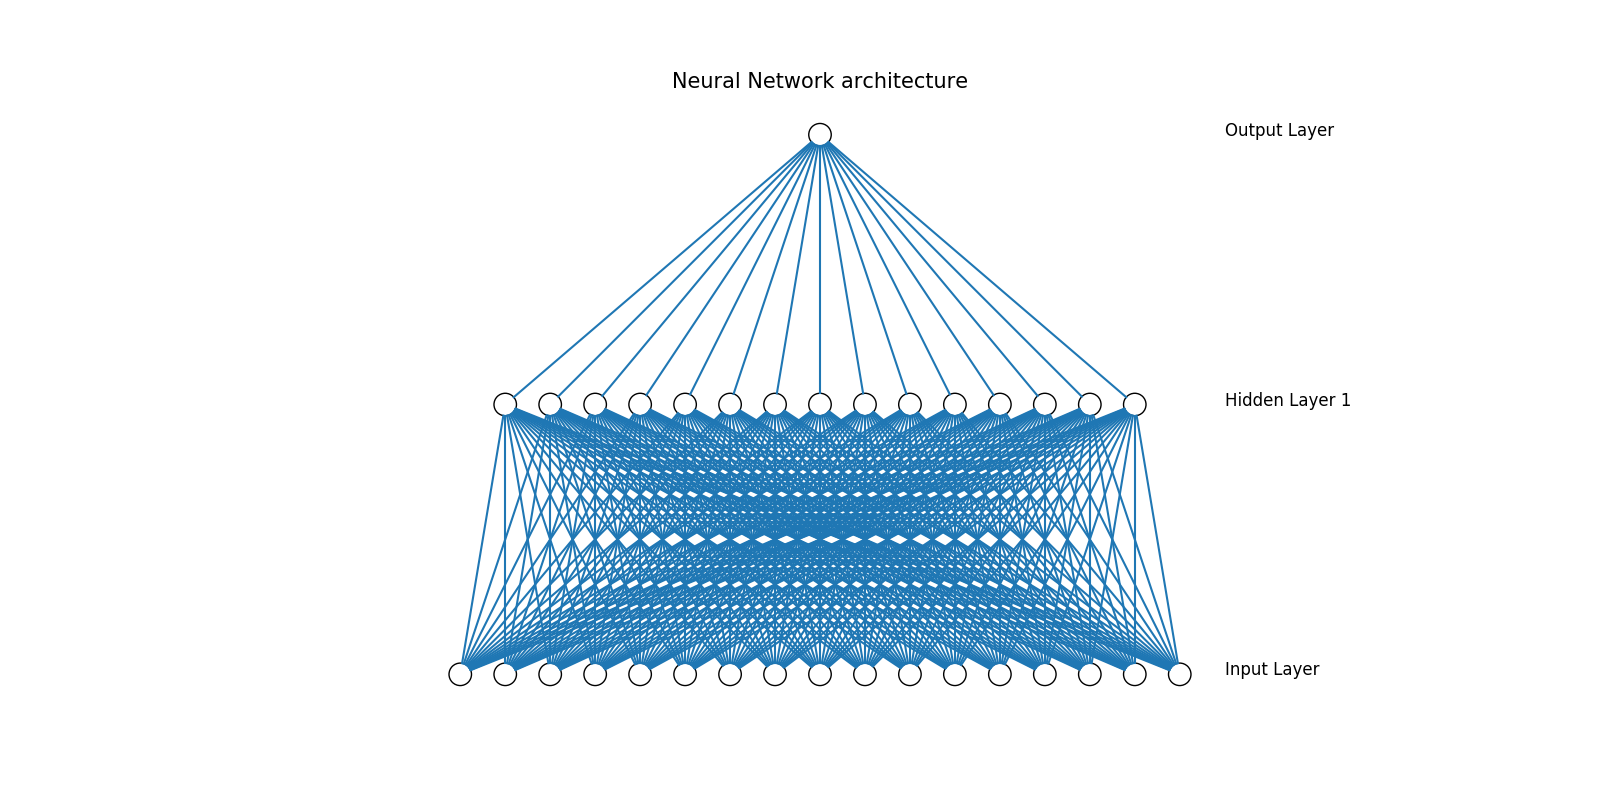
\includegraphics{Experiment2NN.png}

    \begin{Verbatim}[commandchars=\\\{\}]
{\color{incolor}In [{\color{incolor}2}]:} \PY{k}{def} \PY{n+nf}{getNPAnswerArray}\PY{p}{(}\PY{n+nb+bp}{self}\PY{p}{)}\PY{p}{:}
            \PY{c+c1}{\PYZsh{} Char}
            \PY{n}{arr} \PY{o}{=} \PY{n}{np}\PY{o}{.}\PY{n}{array}\PY{p}{(}\PY{p}{[}\PY{p}{[}\PY{l+m+mi}{0}\PY{p}{]}\PY{p}{]}\PY{p}{)}
            \PY{c+c1}{\PYZsh{} Where character is specified. Eg \PYZsq{}A\PYZsq{}}
            \PY{k}{if} \PY{n+nb+bp}{self}\PY{o}{.}\PY{n}{lettr} \PY{o+ow}{in} \PY{n}{\PYZus{}character\PYZus{}match}\PY{p}{:}
                \PY{n}{arr}\PY{p}{[}\PY{l+m+mi}{0}\PY{p}{]}\PY{p}{[}\PY{l+m+mi}{0}\PY{p}{]} \PY{o}{=} \PY{l+m+mi}{1}
            \PY{k}{return} \PY{n}{arr}
\end{Verbatim}


    \hypertarget{tests}{%
\subsection{Tests}\label{tests}}

\hypertarget{nn-configuration}{%
\subsubsection{NN configuration}\label{nn-configuration}}

\begin{longtable}[]{@{}ll@{}}
\toprule
Epochs & Learning rate\tabularnewline
\midrule
\endhead
30 & 0.9\tabularnewline
\bottomrule
\end{longtable}

Momentum tests (Training to recognise the letter `Z'):

\hypertarget{momentum}{%
\paragraph{0.0 Momentum}\label{momentum}}

\begin{verbatim}
======================================
Network stats: 
Learning rate: 0.9
Momentum: 0.0
Epochs: 30
Hidden units: 100
Training error: 1.7525568919432206e-22
Training success: 98.889%
Validation success: 98.901%
======================================
\end{verbatim}

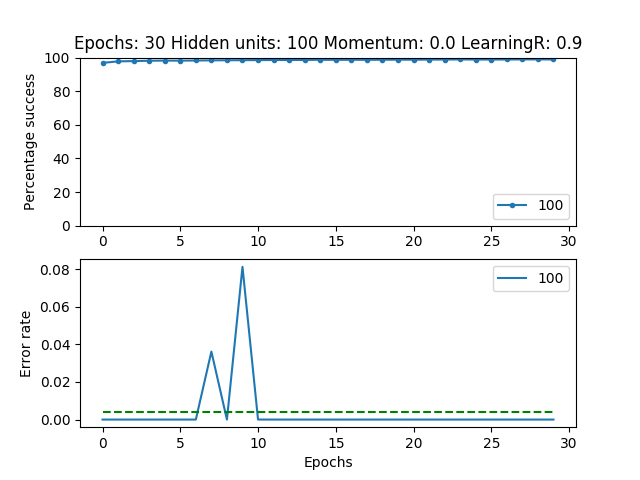
\includegraphics{Experiment1/E1_NN_Epoch_Momentum_0.0_30Epochs_100_LR_0.9_Hiddenunits.png}
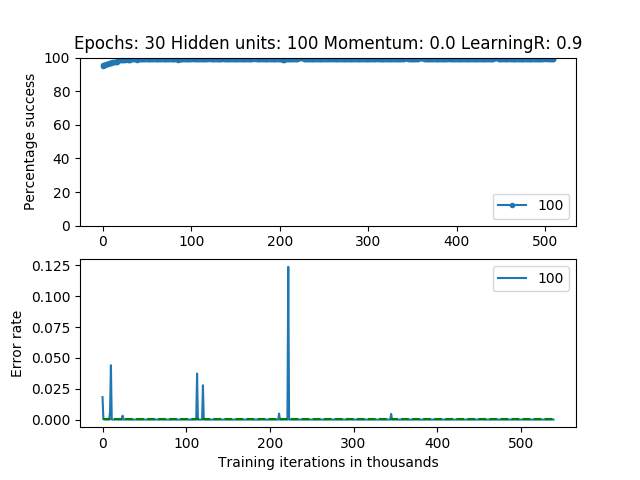
\includegraphics{Experiment1/E1_NN_Training_Momentum_0.0_30Epochs_100_LR_0.9_Hiddenunits.png}

\hypertarget{momentum-1}{%
\paragraph{0.1 Momentum}\label{momentum-1}}

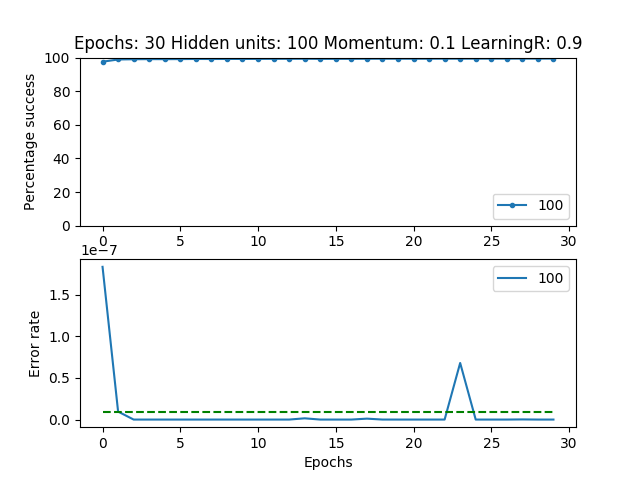
\includegraphics{Experiment1/E1_NN_Epoch_Momentum_0.1_30Epochs_100_LR_0.9_Hiddenunits.png}
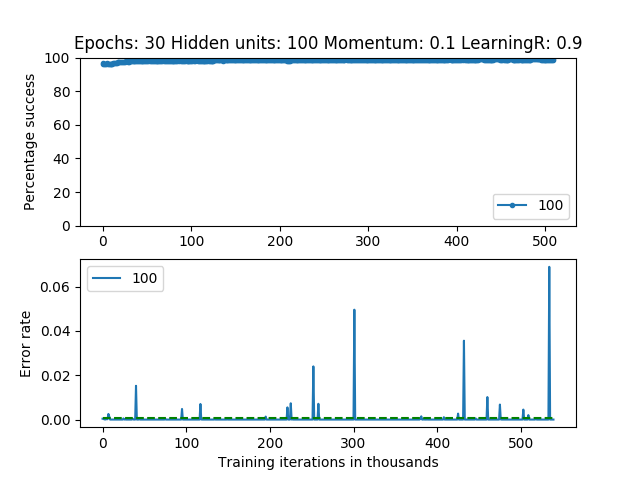
\includegraphics{Experiment1/E1_NN_Training_Momentum_0.1_30Epochs_100_LR_0.9_Hiddenunits.png}

\hypertarget{momentum-2}{%
\paragraph{0.2 Momentum}\label{momentum-2}}

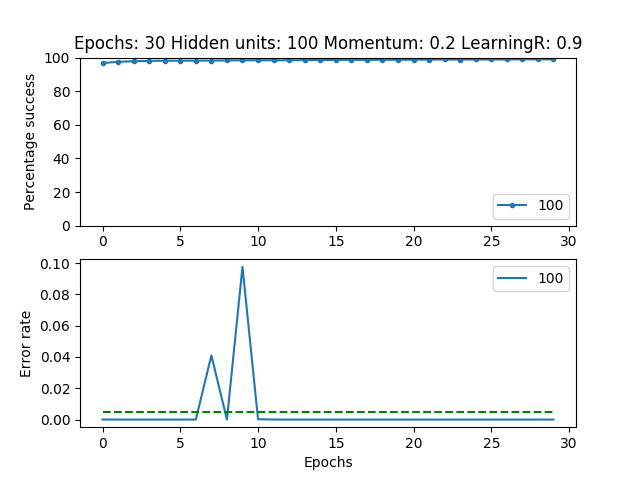
\includegraphics{Experiment1/E1_NN_Epoch_Momentum_0.2_30Epochs_100_LR_0.9_Hiddenunits.png}
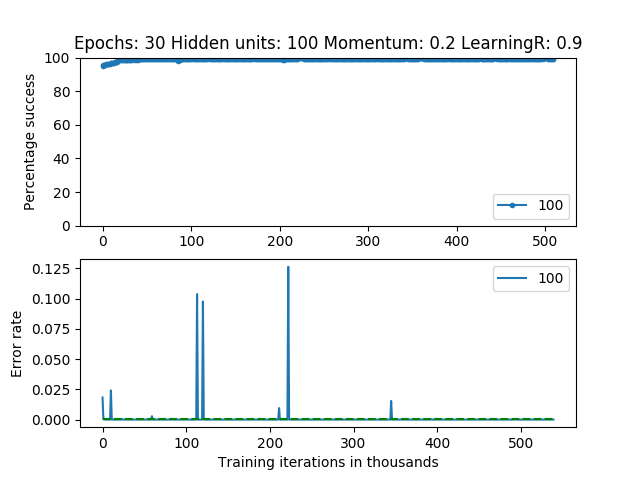
\includegraphics{Experiment1/E1_NN_Training_Momentum_0.2_30Epochs_100_LR_0.9_Hiddenunits.png}

\hypertarget{momentum-3}{%
\paragraph{0.3 Momentum}\label{momentum-3}}

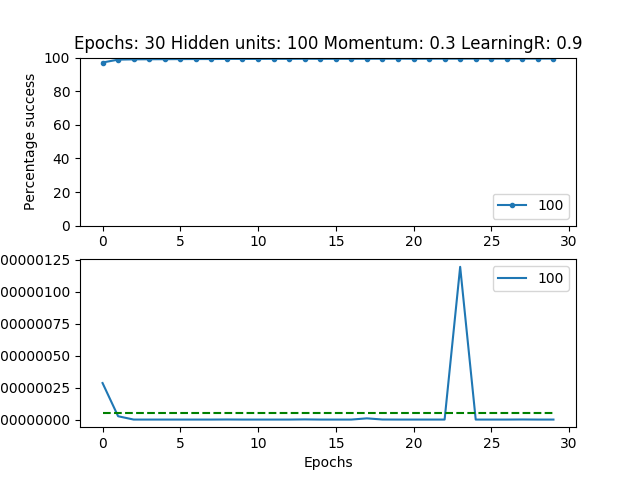
\includegraphics{Experiment1/E1_NN_Epoch_Momentum_0.3_30Epochs_100_LR_0.9_Hiddenunits.png}
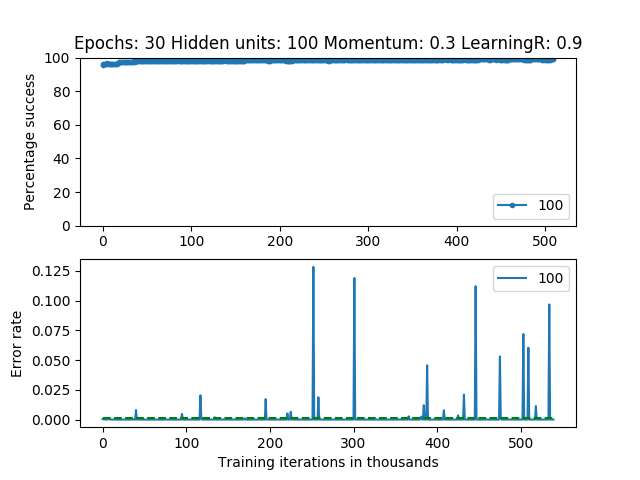
\includegraphics{Experiment1/E1_NN_Training_Momentum_0.3_30Epochs_100_LR_0.9_Hiddenunits.png}

\hypertarget{momentum-4}{%
\paragraph{0.4 Momentum}\label{momentum-4}}

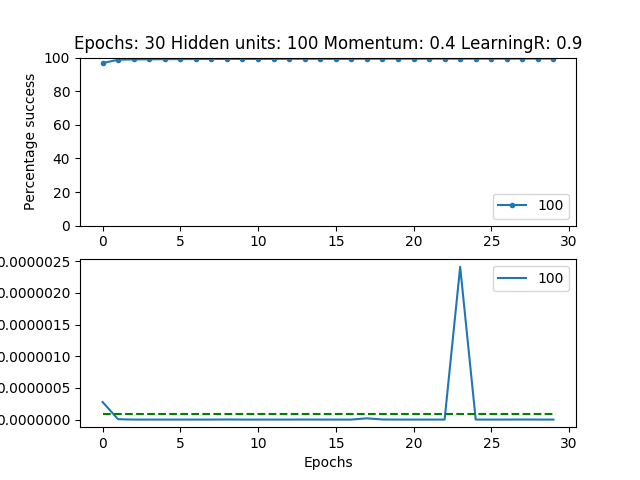
\includegraphics{Experiment1/E1_NN_Epoch_Momentum_0.4_30Epochs_100_LR_0.9_Hiddenunits.png}
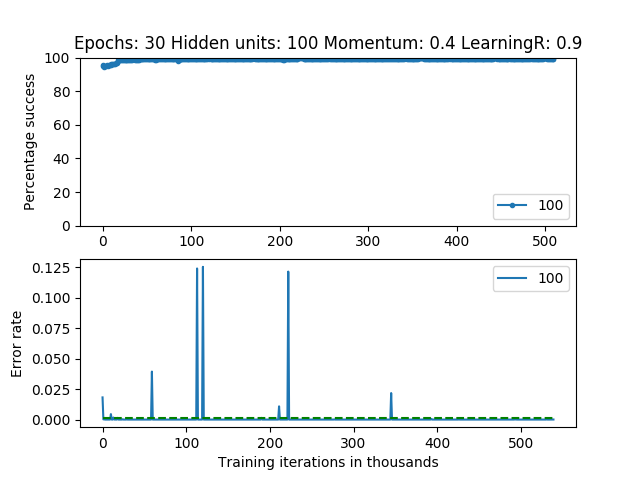
\includegraphics{Experiment1/E1_NN_Training_Momentum_0.4_30Epochs_100_LR_0.9_Hiddenunits.png}

\hypertarget{momentum-5}{%
\paragraph{0.5 Momentum}\label{momentum-5}}

\begin{verbatim}
======================================
Network stats: 
Learning rate: 0.9
Momentum: 0.5
Epochs: 30
Hidden units: 100
Training error: 2.993767961438769e-21
Training success: 98.878%
Validation success: 99.25%
======================================
\end{verbatim}

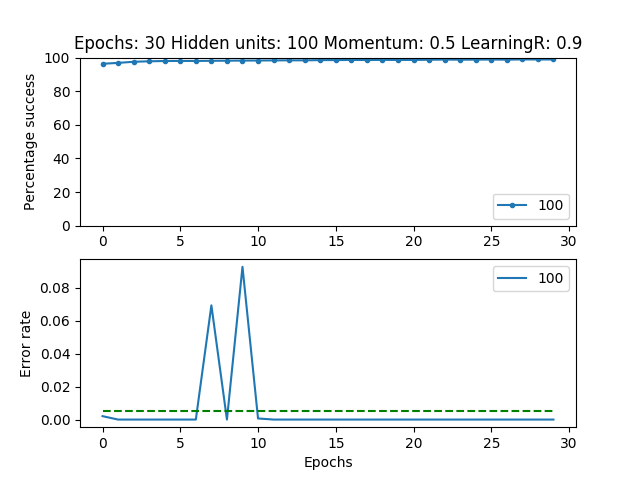
\includegraphics{Experiment1/E1_NN_Epoch_Momentum_0.5_30Epochs_100_LR_0.9_Hiddenunits.png}
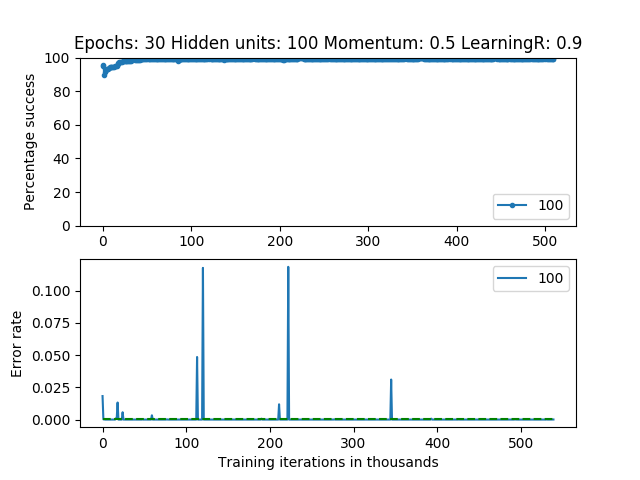
\includegraphics{Experiment1/E1_NN_Training_Momentum_0.5_30Epochs_100_LR_0.9_Hiddenunits.png}

\hypertarget{momentum-6}{%
\paragraph{0.6 Momentum}\label{momentum-6}}

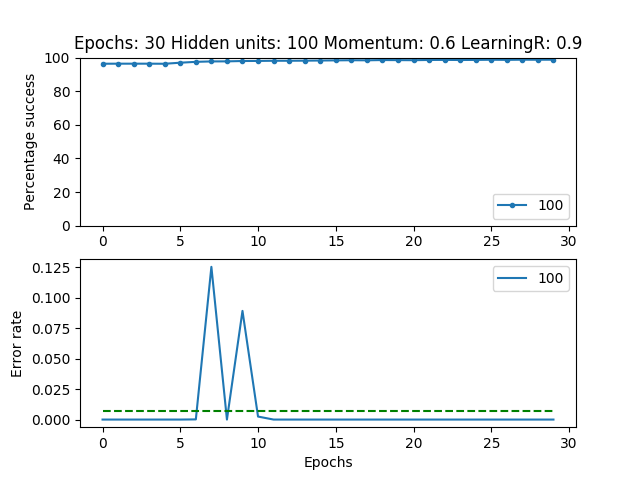
\includegraphics{Experiment1/E1_NN_Epoch_Momentum_0.6_30Epochs_100_LR_0.9_Hiddenunits.png}
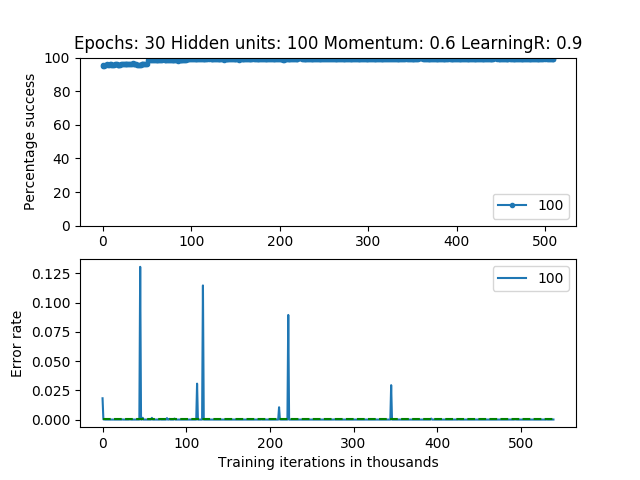
\includegraphics{Experiment1/E1_NN_Training_Momentum_0.6_30Epochs_100_LR_0.9_Hiddenunits.png}

\hypertarget{momentum-7}{%
\paragraph{0.7 Momentum}\label{momentum-7}}

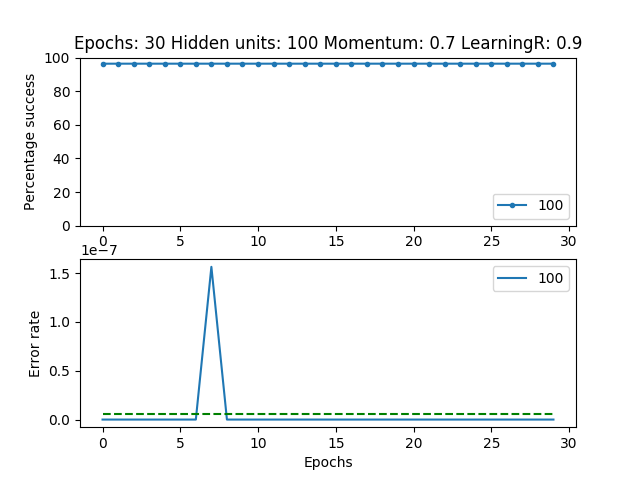
\includegraphics{Experiment1/E1_NN_Epoch_Momentum_0.7_30Epochs_100_LR_0.9_Hiddenunits.png}
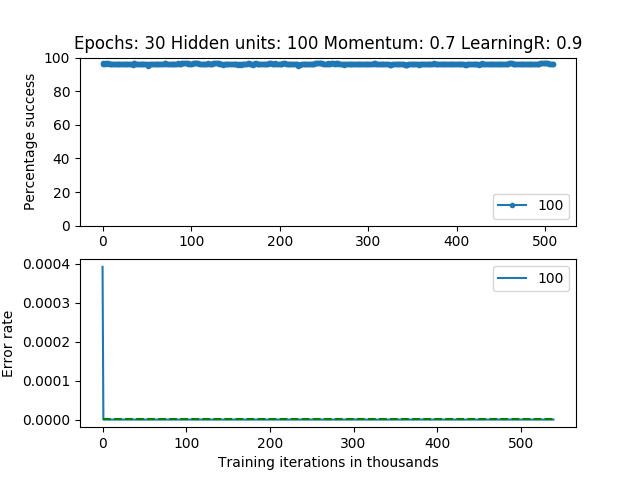
\includegraphics{Experiment1/E1_NN_Training_Momentum_0.7_30Epochs_100_LR_0.9_Hiddenunits.png}

\hypertarget{momentum-8}{%
\paragraph{0.8 Momentum}\label{momentum-8}}

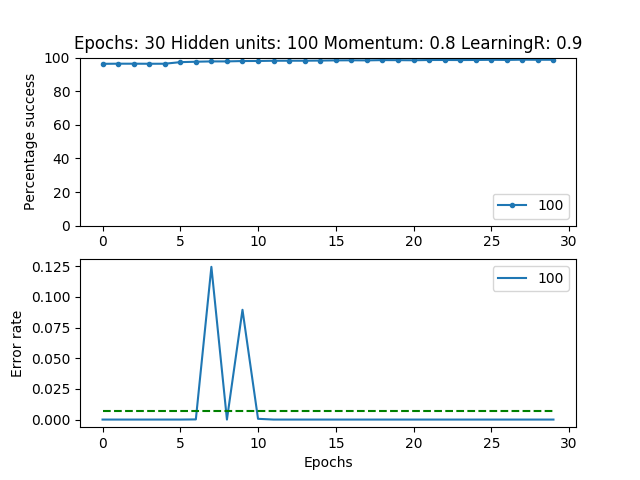
\includegraphics{Experiment1/E1_NN_Epoch_Momentum_0.8_30Epochs_100_LR_0.9_Hiddenunits.png}
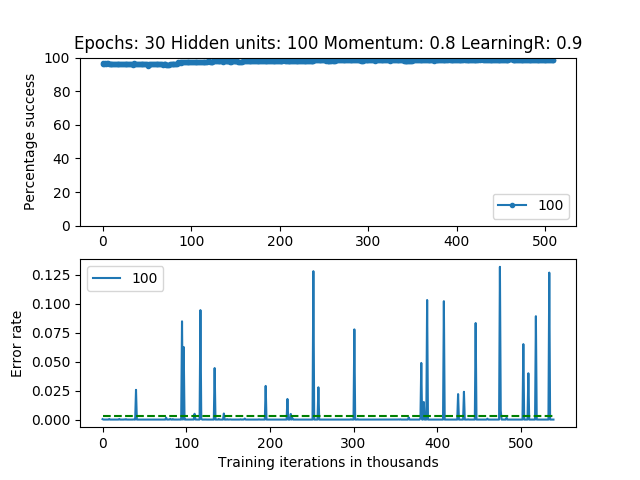
\includegraphics{Experiment1/E1_NN_Training_Momentum_0.8_30Epochs_100_LR_0.9_Hiddenunits.png}

\hypertarget{momentum-9}{%
\paragraph{0.9 Momentum}\label{momentum-9}}

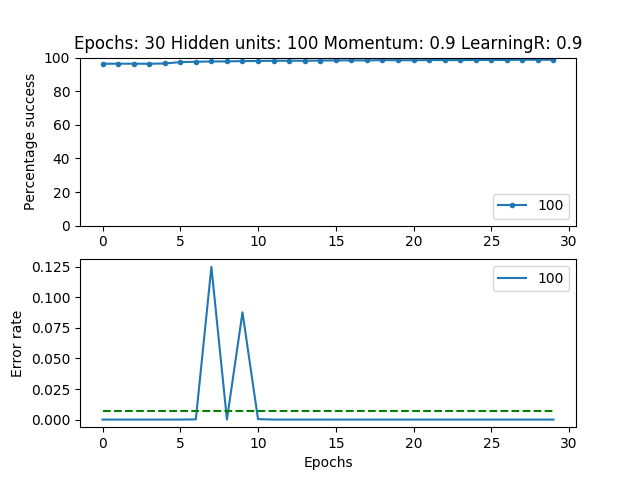
\includegraphics{Experiment1/E1_NN_Epoch_Momentum_0.9_30Epochs_100_LR_0.9_Hiddenunits.png}
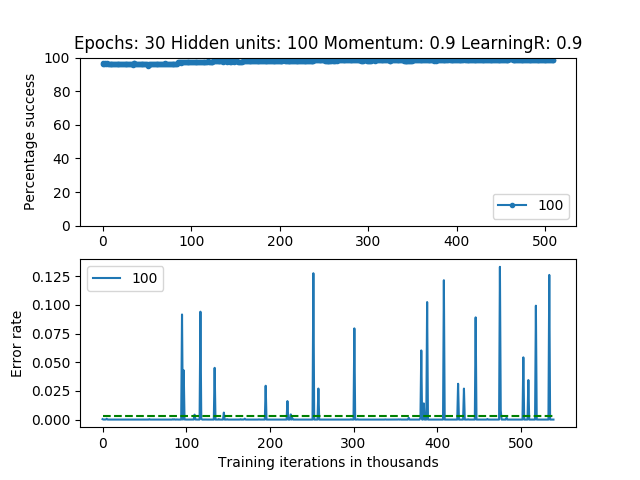
\includegraphics{Experiment1/E1_NN_Training_Momentum_0.9_30Epochs_100_LR_0.9_Hiddenunits.png}

\hypertarget{momentum-10}{%
\paragraph{1.0 Momentum}\label{momentum-10}}

\begin{verbatim}
======================================
Network stats: 
Learning rate: 0.9
Momentum: 1.0
Epochs: 30
Hidden units: 100
Training error: 5.0668758290754695e-14
Training success: 96.383%
Validation success: 95.902%
======================================
\end{verbatim}

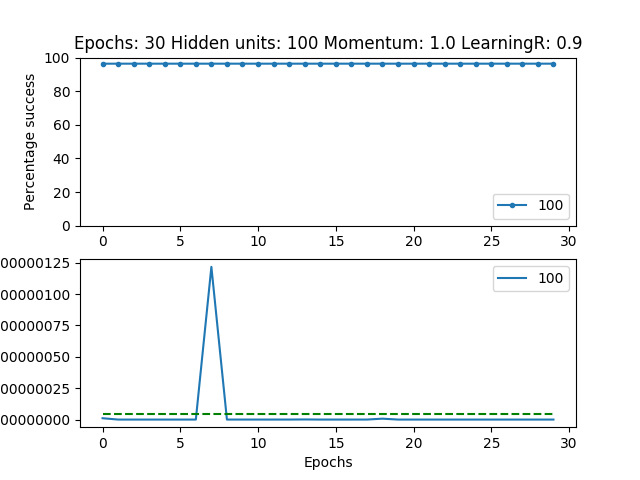
\includegraphics{Experiment1/E1_NN_Epoch_Momentum_1.0_30Epochs_100_LR_0.9_Hiddenunits.png}
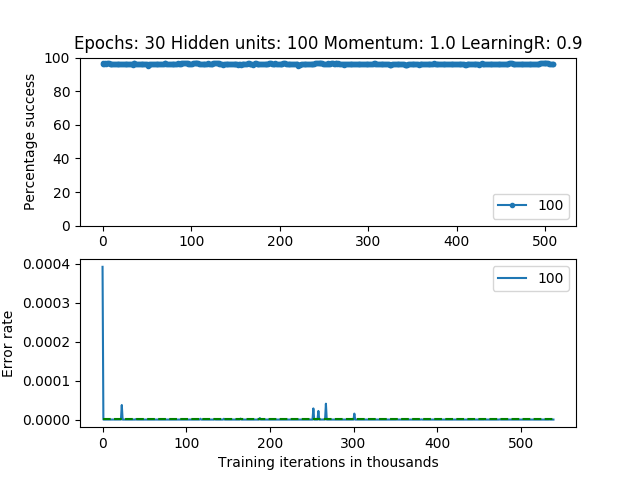
\includegraphics{Experiment1/E1_NN_Training_Momentum_1.0_30Epochs_100_LR_0.9_Hiddenunits.png}

\hypertarget{nn-configuration-1}{%
\subsubsection{NN configuration}\label{nn-configuration-1}}

Based on the previous tests a lower momentum gave better results. So
0.01 was chosen as the momentum and now tests were run to see what
learning rate was ideal.

\begin{longtable}[]{@{}ll@{}}
\toprule
Epochs & Momentum\tabularnewline
\midrule
\endhead
30 & 0.01\tabularnewline
\bottomrule
\end{longtable}

\hypertarget{learning-rate}{%
\paragraph{0.1 Learning rate}\label{learning-rate}}

\begin{verbatim}
======================================
Network stats: 
Learning rate: 0.1
Momentum: 0.01
Epochs: 30
Hidden units: 100
Training error: 6.717862098369651e-09
Training success: 98.2%
Validation success: 98.401%
======================================
\end{verbatim}

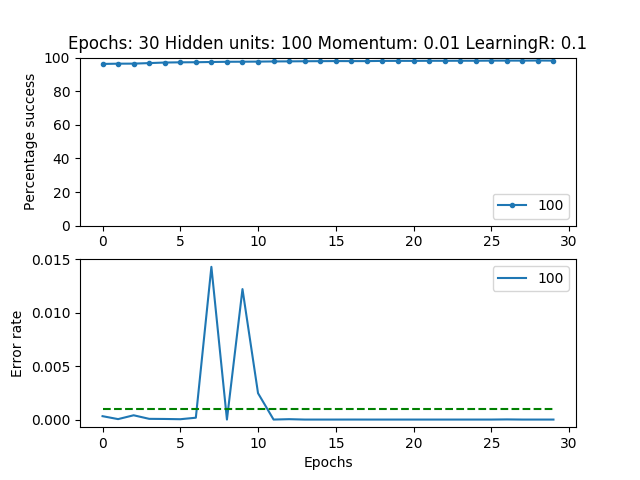
\includegraphics{Experiment1/E1_NN_Epoch_Momentum_0.01_30Epochs_100_LR_0.1_Hiddenunits.png}
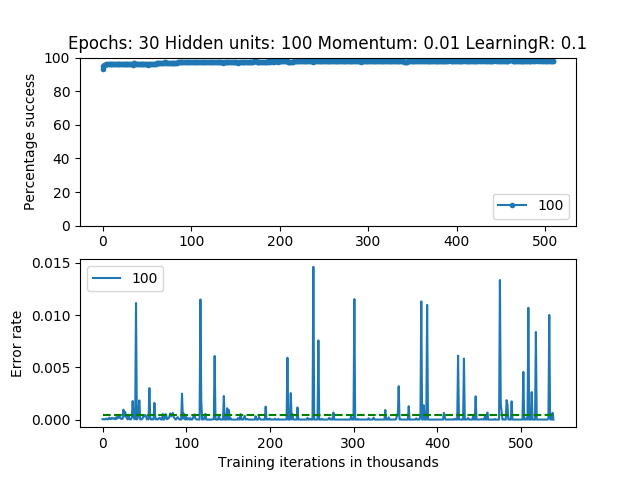
\includegraphics{Experiment1/E1_NN_Training_Momentum_0.01_30Epochs_100_LR_0.1_Hiddenunits.png}

\hypertarget{learning-rate-1}{%
\paragraph{0.2 Learning rate}\label{learning-rate-1}}

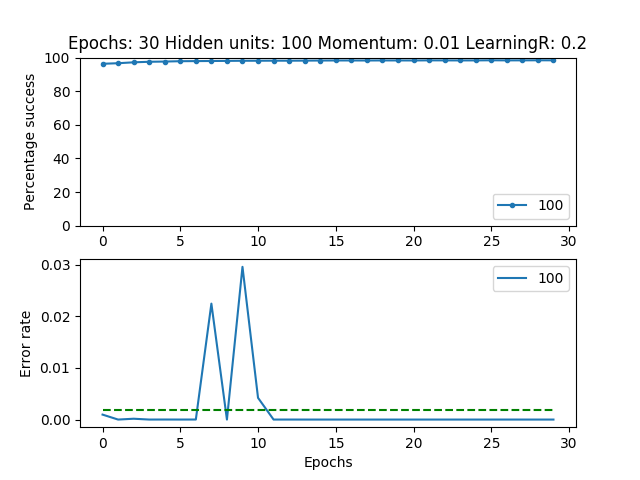
\includegraphics{Experiment1/E1_NN_Epoch_Momentum_0.01_30Epochs_100_LR_0.2_Hiddenunits.png}
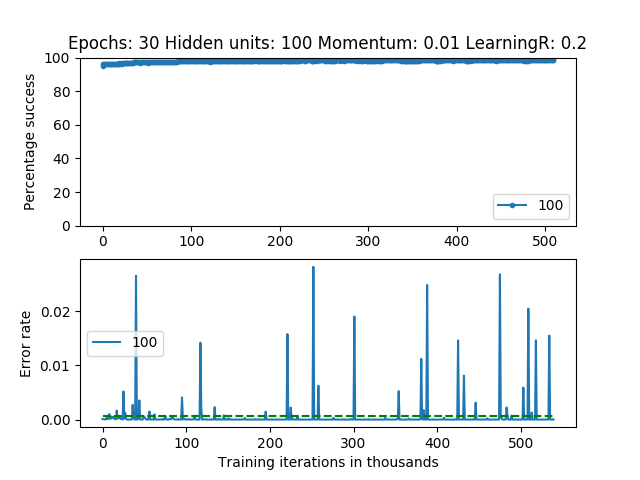
\includegraphics{Experiment1/E1_NN_Training_Momentum_0.01_30Epochs_100_LR_0.2_Hiddenunits.png}

\hypertarget{learning-rate-2}{%
\paragraph{0.3 Learning rate}\label{learning-rate-2}}

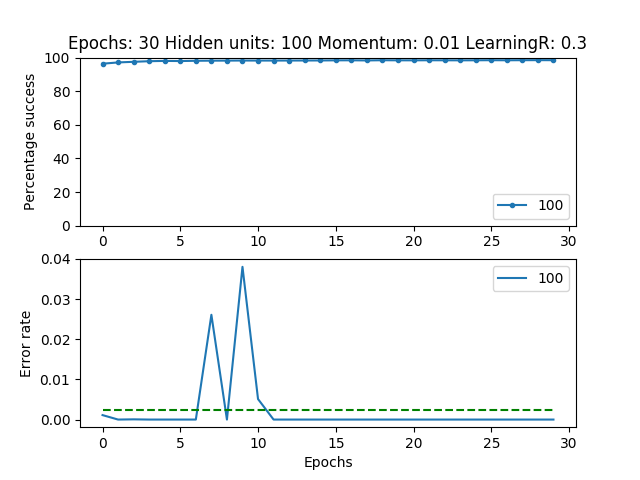
\includegraphics{Experiment1/E1_NN_Epoch_Momentum_0.01_30Epochs_100_LR_0.3_Hiddenunits.png}
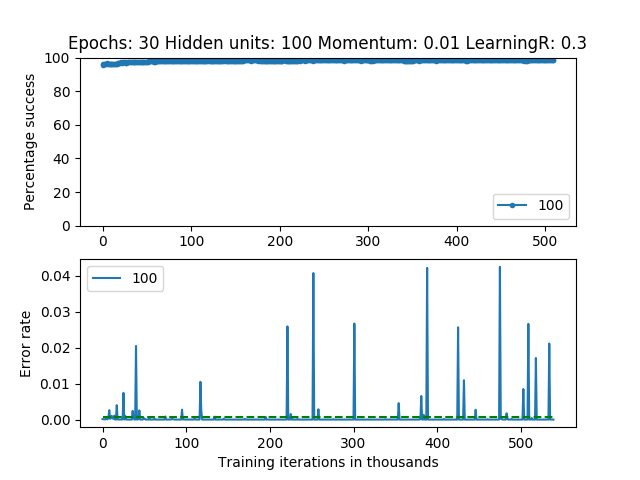
\includegraphics{Experiment1/E1_NN_Training_Momentum_0.01_30Epochs_100_LR_0.3_Hiddenunits.png}

\hypertarget{learning-rate-3}{%
\paragraph{0.4 Learning rate}\label{learning-rate-3}}

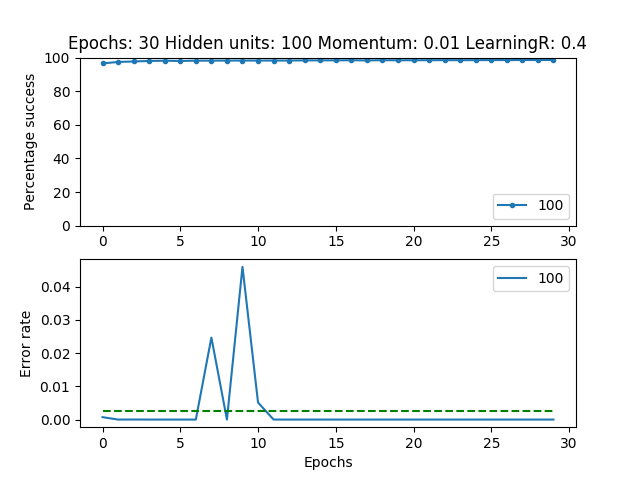
\includegraphics{Experiment1/E1_NN_Epoch_Momentum_0.01_30Epochs_100_LR_0.4_Hiddenunits.png}
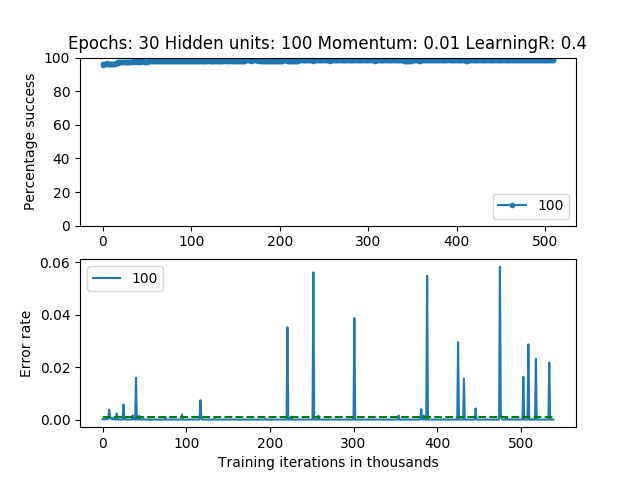
\includegraphics{Experiment1/E1_NN_Training_Momentum_0.01_30Epochs_100_LR_0.4_Hiddenunits.png}

\hypertarget{learning-rate-4}{%
\paragraph{0.5 Learning rate}\label{learning-rate-4}}

\begin{verbatim}
======================================
Network stats: 
Learning rate: 0.5
Momentum: 0.01
Epochs: 30
Hidden units: 100
Training error: 2.1486977050637392e-17
Training success: 98.711%
Validation success: 99.0%
======================================
\end{verbatim}

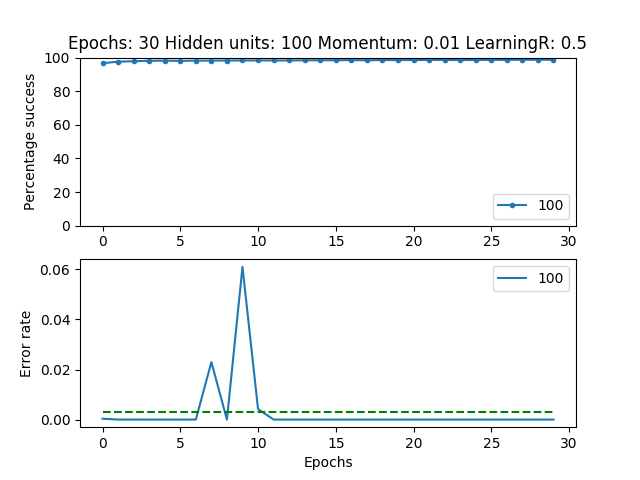
\includegraphics{Experiment1/E1_NN_Epoch_Momentum_0.01_30Epochs_100_LR_0.5_Hiddenunits.png}
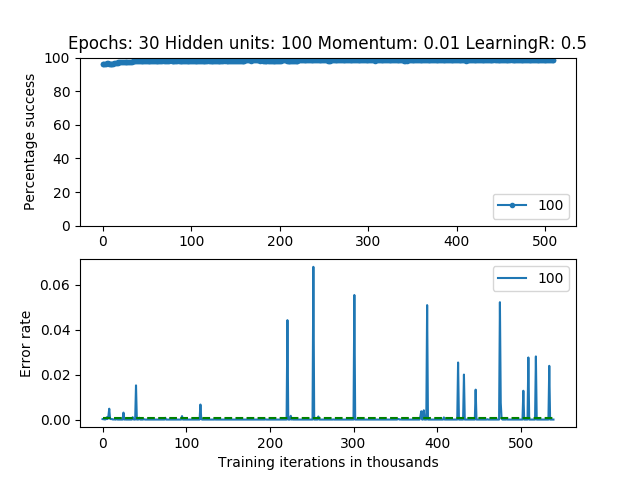
\includegraphics{Experiment1/E1_NN_Training_Momentum_0.01_30Epochs_100_LR_0.5_Hiddenunits.png}

\hypertarget{learning-rate-5}{%
\paragraph{0.6 Learning rate}\label{learning-rate-5}}

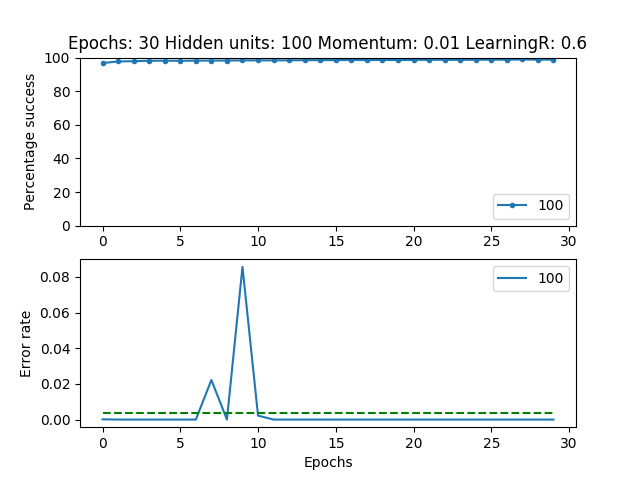
\includegraphics{Experiment1/E1_NN_Epoch_Momentum_0.01_30Epochs_100_LR_0.6_Hiddenunits.png}
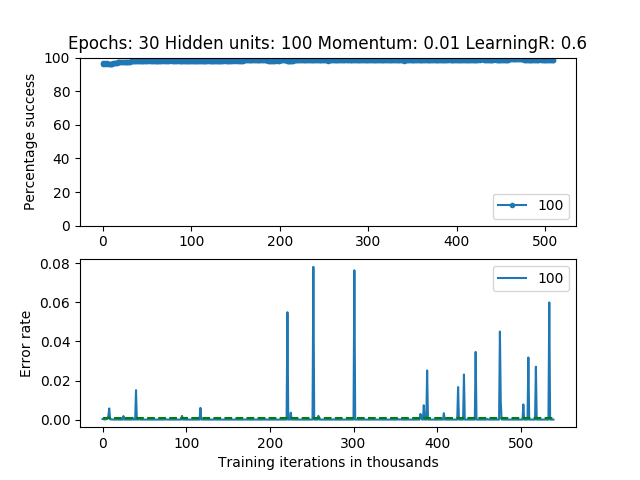
\includegraphics{Experiment1/E1_NN_Training_Momentum_0.01_30Epochs_100_LR_0.6_Hiddenunits.png}

\hypertarget{learning-rate-6}{%
\paragraph{0.7 Learning rate}\label{learning-rate-6}}

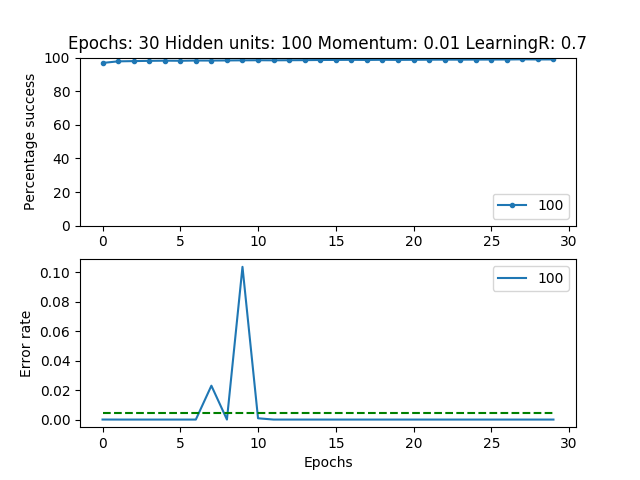
\includegraphics{Experiment1/E1_NN_Epoch_Momentum_0.01_30Epochs_100_LR_0.7_Hiddenunits.png}
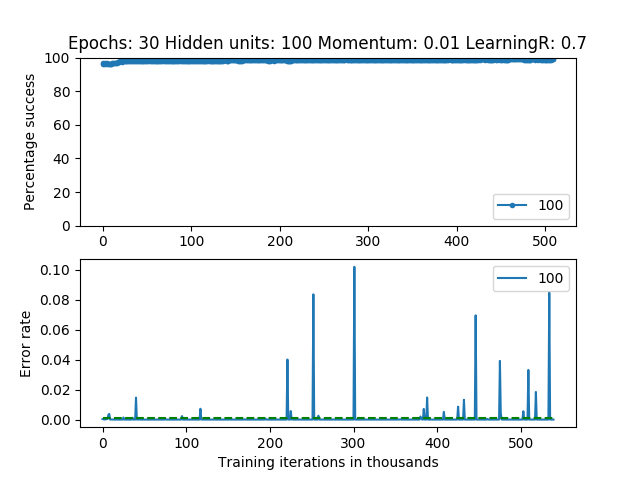
\includegraphics{Experiment1/E1_NN_Training_Momentum_0.01_30Epochs_100_LR_0.7_Hiddenunits.png}

\hypertarget{learning-rate-7}{%
\paragraph{0.8 Learning rate}\label{learning-rate-7}}

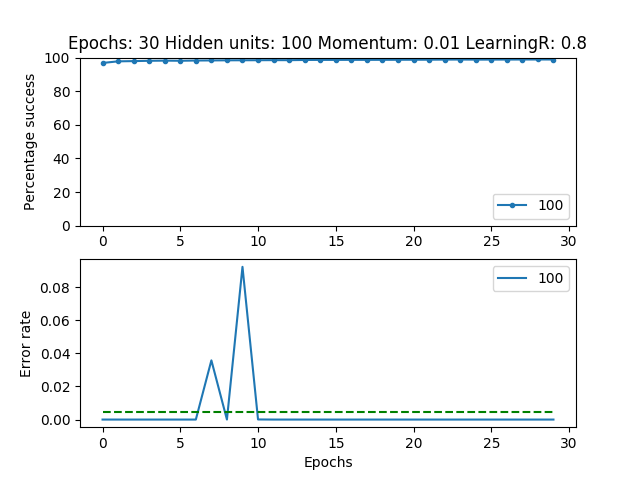
\includegraphics{Experiment1/E1_NN_Epoch_Momentum_0.01_30Epochs_100_LR_0.8_Hiddenunits.png}
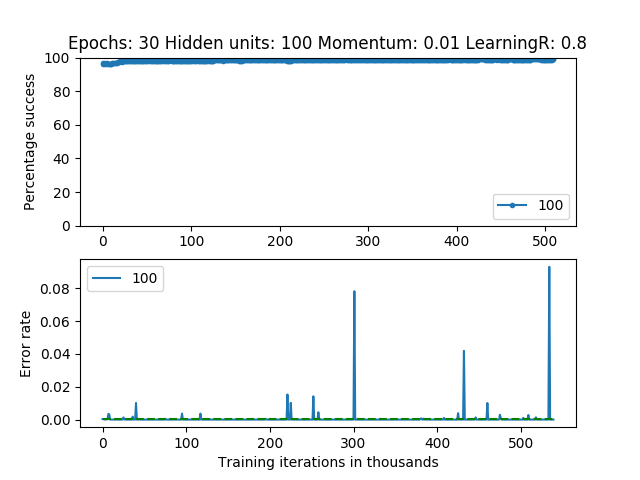
\includegraphics{Experiment1/E1_NN_Training_Momentum_0.01_30Epochs_100_LR_0.8_Hiddenunits.png}

\hypertarget{learning-rate-8}{%
\paragraph{0.9 Learning rate}\label{learning-rate-8}}

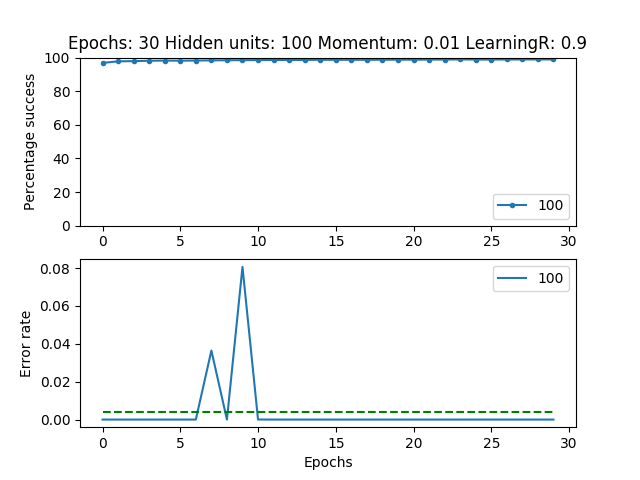
\includegraphics{Experiment1/E1_NN_Epoch_Momentum_0.01_30Epochs_100_LR_0.9_Hiddenunits.png}
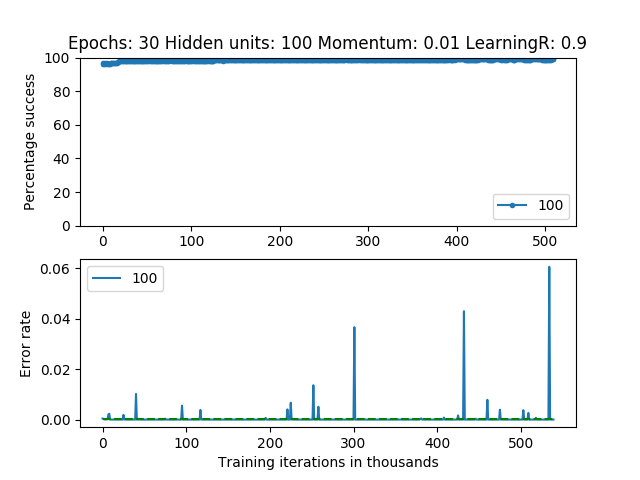
\includegraphics{Experiment1/E1_NN_Training_Momentum_0.01_30Epochs_100_LR_0.9_Hiddenunits.png}

\hypertarget{learning-rate-9}{%
\paragraph{1.0 Learning rate}\label{learning-rate-9}}

\begin{verbatim}
======================================
Network stats: 
Learning rate: 1.0
Momentum: 0.01
Epochs: 30
Hidden units: 100
Training error: 6.921868880478976e-24
Training success: 98.928%
Validation success: 99.05%
======================================
\end{verbatim}

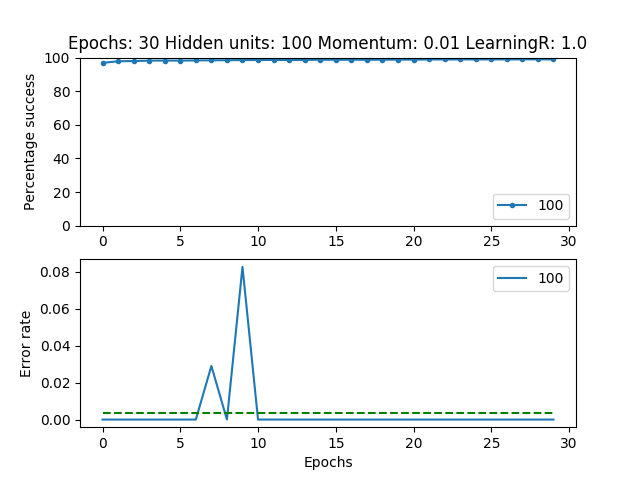
\includegraphics{Experiment1/E1_NN_Epoch_Momentum_0.01_30Epochs_100_LR_1.0_Hiddenunits.png}
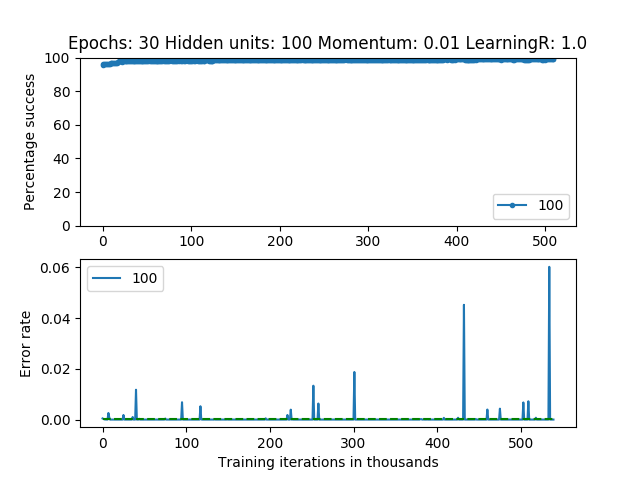
\includegraphics{Experiment1/E1_NN_Training_Momentum_0.01_30Epochs_100_LR_1.0_Hiddenunits.png}

\hypertarget{best-result}{%
\subsection{Best result}\label{best-result}}

\begin{verbatim}
======================================
Network stats: 
Learning rate: 1.0
Momentum: 0.01
Epochs: 30
Hidden units: 100
Training error: 6.921868880478976e-24
Training success: 98.928%
Validation success: 99.05%
======================================
\end{verbatim}

The higher learning rate reached the highest training generalization and
highest validation success.

\hypertarget{conclusion}{%
\subsection{Conclusion}\label{conclusion}}

A low momentum and a high learning rate gave the best generalization
results.

    \hypertarget{experiment-2}{%
\section{Experiment 2}\label{experiment-2}}

\begin{longtable}[]{@{}lll@{}}
\toprule
Student nmr & Name & Date\tabularnewline
\midrule
\endhead
15015026 & Thomas Scholtz & 23 May 2018\tabularnewline
\bottomrule
\end{longtable}

To run experiment 2: \texttt{python\ experiment2.py}

    \hypertarget{data-preprocessing}{%
\subsection{Data preprocessing}\label{data-preprocessing}}

\hypertarget{numerical-preprocessing}{%
\subsubsection{Numerical preprocessing}\label{numerical-preprocessing}}

For numerical values the data was normalised to {[}0-1{]}. (Min-max
normalization).

\begin{verbatim}
Example Numerical preprocessing
Scaled: 2   to: 0.13333333333333333
Scaled: 8   to: 0.5333333333333333
Scaled: 3   to: 0.2
Scaled: 5   to: 0.3333333333333333
Scaled: 1   to: 0.06666666666666667
Scaled: 8   to: 0.5333333333333333
Scaled: 13  to: 0.8666666666666667
Scaled: 0   to: 0.0
Scaled: 6   to: 0.4
Scaled: 6   to: 0.4
Scaled: 10  to: 0.6666666666666666
Scaled: 8   to: 0.5333333333333333
Scaled: 0   to: 0.0
Scaled: 8   to: 0.5333333333333333
Scaled: 0   to: 0.0
Scaled: 8   to: 0.5333333333333333
\end{verbatim}

\hypertarget{character-preprocessing}{%
\subsubsection{Character preprocessing}\label{character-preprocessing}}

For the characters the data was first converted to lower case, then to
the ascii number and finally 97 was subtracted.

\begin{verbatim}
Example character preprocessing
Scaled: A   to: 0
Scaled: B   to: 1
Scaled: C   to: 2
Scaled: D   to: 3
Scaled: E   to: 4
Scaled: F   to: 5
Scaled: Z   to: 25
\end{verbatim}

For the training data a corresponding 0 or 1 was given as the answer for
the training data.

    \hypertarget{data-split}{%
\subsection{Data split}\label{data-split}}

For training I used 18000 of the 20000 entries given for training the
neural network. The remainder of the data was used to validate the
neural network.

\hypertarget{stopping-conditions}{%
\subsection{Stopping conditions}\label{stopping-conditions}}

\begin{itemize}
\tightlist
\item
  When a maximum number of epochs is exceeded
\item
  When the generalization error, E G , is acceptable
\end{itemize}

\hypertarget{network-architecture}{%
\subsection{Network Architecture}\label{network-architecture}}

The architecture consists of 17 input neurons (including bias), 100
hidden units and 1 output unit. 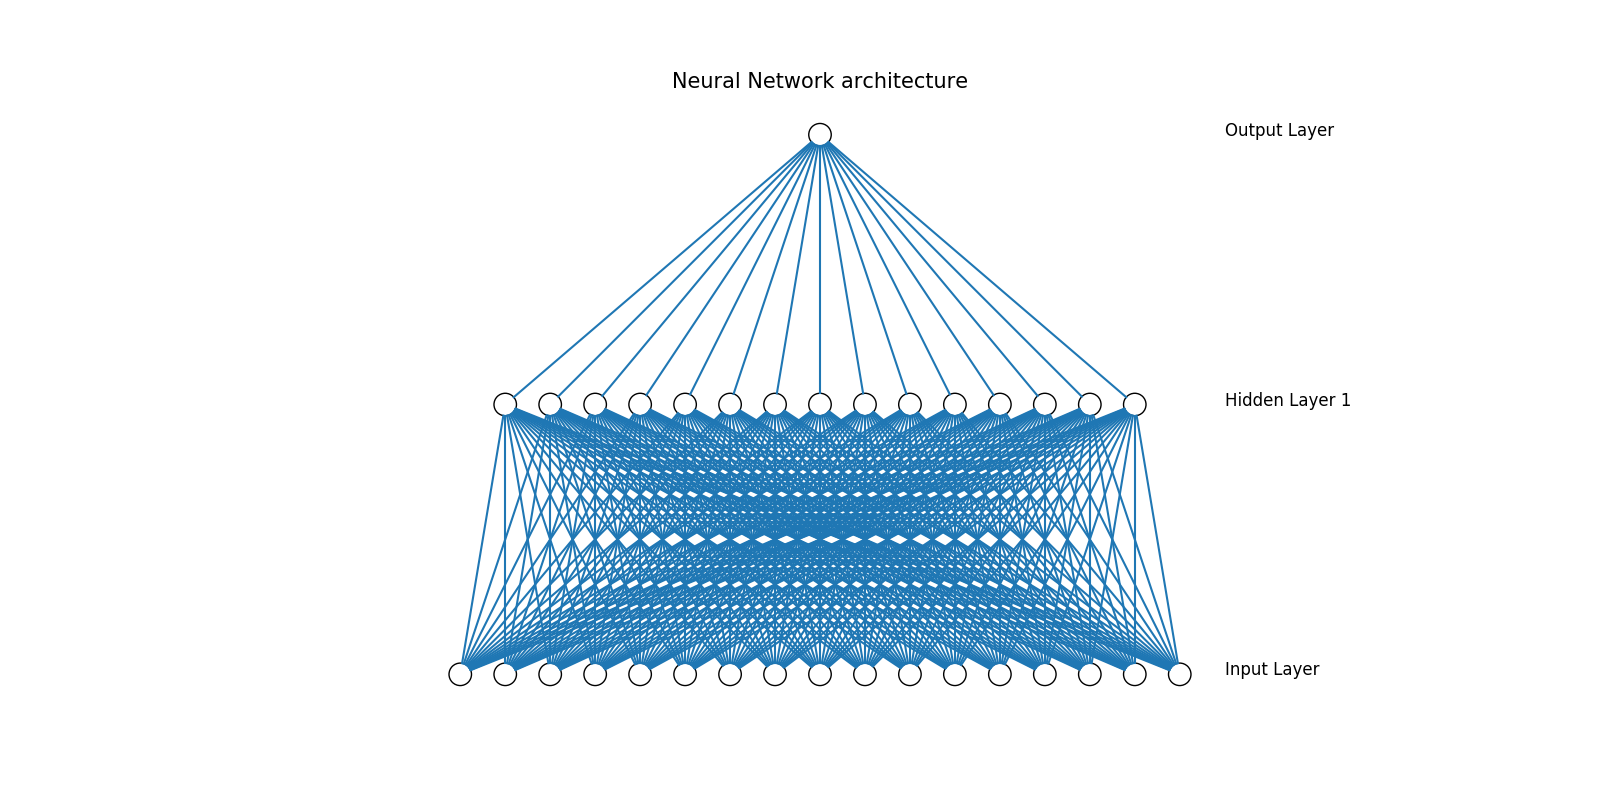
\includegraphics{Experiment2NN.png}

    \begin{Verbatim}[commandchars=\\\{\}]
{\color{incolor}In [{\color{incolor}1}]:} \PY{k}{def} \PY{n+nf}{getNPAnswerArray}\PY{p}{(}\PY{n+nb+bp}{self}\PY{p}{)}\PY{p}{:}
            \PY{c+c1}{\PYZsh{} Vowels}
            \PY{n}{arr} \PY{o}{=} \PY{n}{np}\PY{o}{.}\PY{n}{array}\PY{p}{(}\PY{p}{[}\PY{p}{[}\PY{l+m+mi}{0}\PY{p}{]}\PY{p}{]}\PY{p}{)}
        
            \PY{k}{if} \PY{n+nb+bp}{self}\PY{o}{.}\PY{n}{lettr} \PY{o+ow}{in} \PY{l+s+s2}{\PYZdq{}}\PY{l+s+s2}{AEIOU}\PY{l+s+s2}{\PYZdq{}}\PY{p}{:}
                \PY{n}{arr}\PY{p}{[}\PY{l+m+mi}{0}\PY{p}{]}\PY{p}{[}\PY{l+m+mi}{0}\PY{p}{]} \PY{o}{=} \PY{l+m+mi}{1}
            \PY{k}{return} \PY{n}{arr}
\end{Verbatim}


    \hypertarget{tests}{%
\subsection{Tests}\label{tests}}

\hypertarget{nn-configuration}{%
\subsubsection{NN configuration}\label{nn-configuration}}

\begin{longtable}[]{@{}ll@{}}
\toprule
Epochs & Learning rate\tabularnewline
\midrule
\endhead
30 & 0.9\tabularnewline
\bottomrule
\end{longtable}

    \hypertarget{momentum}{%
\paragraph{0.0 Momentum}\label{momentum}}

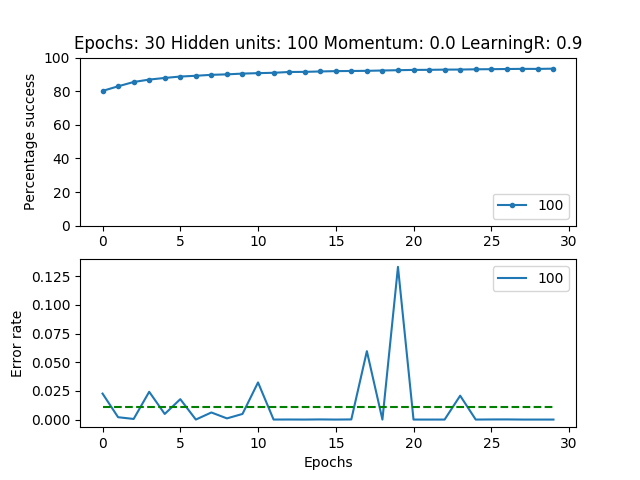
\includegraphics{Experiment2/E2_NN_Epoch_Momentum_0.0_30Epochs_100Hiddenunits.png}
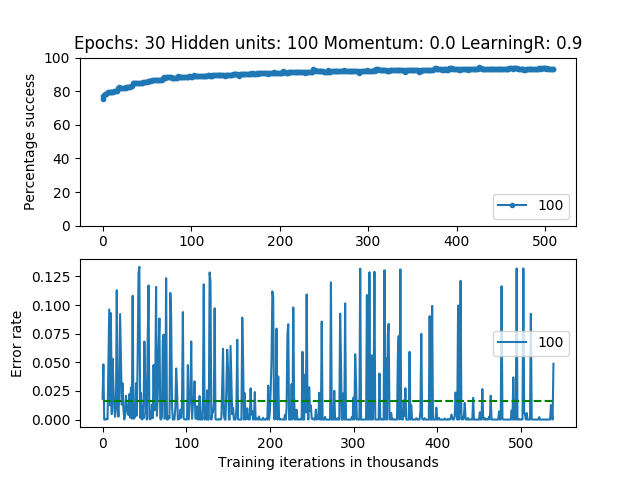
\includegraphics{Experiment2/E2_NN_Training_Momentum_0.0_30Epochs_100Hiddenunits.png}

\hypertarget{momentum-1}{%
\paragraph{0.1 Momentum}\label{momentum-1}}

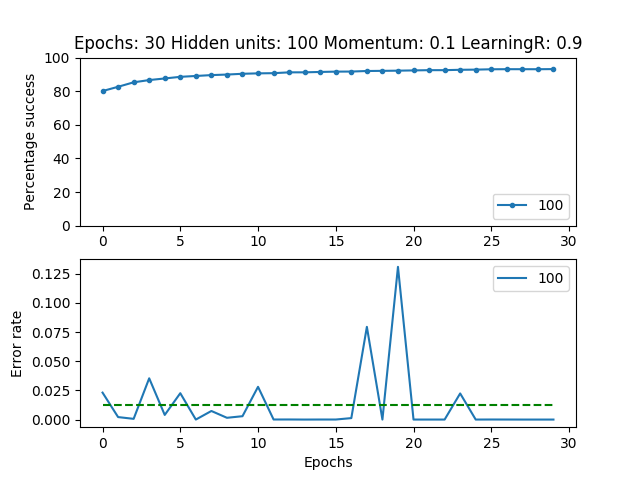
\includegraphics{Experiment2/E2_NN_Epoch_Momentum_0.1_30Epochs_100Hiddenunits.png}
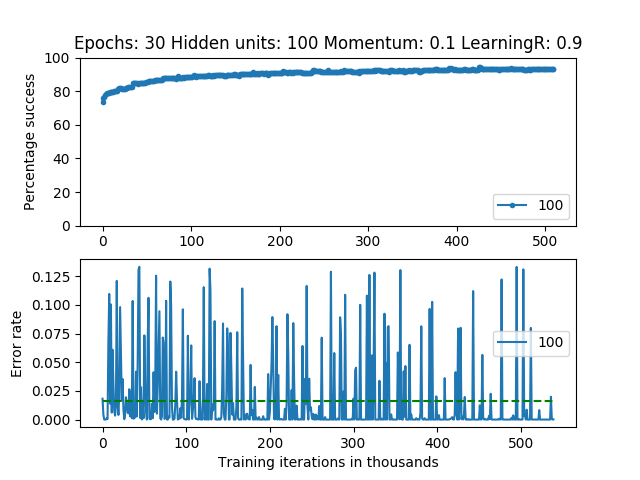
\includegraphics{Experiment2/E2_NN_Training_Momentum_0.1_30Epochs_100Hiddenunits.png}

\hypertarget{momentum-2}{%
\paragraph{0.2 Momentum}\label{momentum-2}}

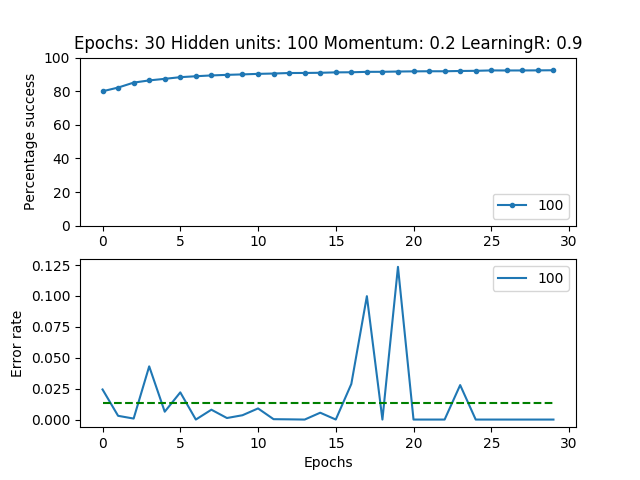
\includegraphics{Experiment2/E2_NN_Epoch_Momentum_0.2_30Epochs_100Hiddenunits.png}
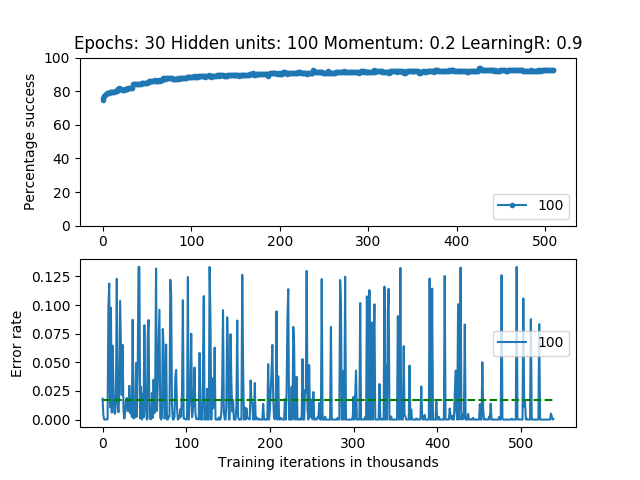
\includegraphics{Experiment2/E2_NN_Training_Momentum_0.2_30Epochs_100Hiddenunits.png}

\hypertarget{momentum-3}{%
\paragraph{0.3 Momentum}\label{momentum-3}}

\includegraphics{Experiment2/E2_NN_Epoch_Momentum_0.3_30Epochs_100Hiddenunits.png}
\includegraphics{Experiment2/E2_NN_Training_Momentum_0.3_30Epochs_100Hiddenunits.png}

\hypertarget{momentum-4}{%
\paragraph{0.4 Momentum}\label{momentum-4}}

\includegraphics{Experiment2/E2_NN_Epoch_Momentum_0.4_30Epochs_100Hiddenunits.png}
\includegraphics{Experiment2/E2_NN_Training_Momentum_0.4_30Epochs_100Hiddenunits.png}

\hypertarget{momentum-5}{%
\paragraph{0.5 Momentum}\label{momentum-5}}

\includegraphics{Experiment2/E2_NN_Epoch_Momentum_0.5_30Epochs_100Hiddenunits.png}
\includegraphics{Experiment2/E2_NN_Training_Momentum_0.5_30Epochs_100Hiddenunits.png}

\hypertarget{momentum-6}{%
\paragraph{0.6 Momentum}\label{momentum-6}}

\includegraphics{Experiment2/E2_NN_Epoch_Momentum_0.6_30Epochs_100Hiddenunits.png}
\includegraphics{Experiment2/E2_NN_Training_Momentum_0.6_30Epochs_100Hiddenunits.png}

\hypertarget{momentum-7}{%
\paragraph{0.7 Momentum}\label{momentum-7}}

\includegraphics{Experiment2/E2_NN_Epoch_Momentum_0.7_30Epochs_100Hiddenunits.png}
\includegraphics{Experiment2/E2_NN_Training_Momentum_0.7_30Epochs_100Hiddenunits.png}

\hypertarget{momentum-8}{%
\paragraph{0.8 Momentum}\label{momentum-8}}

\includegraphics{Experiment2/E2_NN_Epoch_Momentum_0.8_30Epochs_100Hiddenunits.png}
\includegraphics{Experiment2/E2_NN_Training_Momentum_0.8_30Epochs_100Hiddenunits.png}

\hypertarget{momentum-9}{%
\paragraph{0.9 Momentum}\label{momentum-9}}

\includegraphics{Experiment2/E2_NN_Epoch_Momentum_0.9_30Epochs_100Hiddenunits.png}
\includegraphics{Experiment2/E2_NN_Training_Momentum_0.9_30Epochs_100Hiddenunits.png}

\hypertarget{momentum-10}{%
\paragraph{1.0 Momentum}\label{momentum-10}}

\begin{verbatim}
======================================
Network stats: 
Learning rate: 0.9
Momentum: 1.0
Epochs: 30
Hidden units: 100
Training error: 0.000190781674932777
Training success: 80.667%
Validation success: 80.11%
======================================
\end{verbatim}

\includegraphics{Experiment2/E2_NN_Epoch_Momentum_1.0_30Epochs_100Hiddenunits.png}
\includegraphics{Experiment2/E2_NN_Training_Momentum_1.0_30Epochs_100Hiddenunits.png}

\hypertarget{best-result}{%
\subsection{Best result}\label{best-result}}

\begin{verbatim}
======================================
This NN is still best:
======================================
Network stats: 
Learning rate: 0.9
Momentum: 0.0
Epochs: 30
Hidden units: 100
Training error: 2.9226455776084096e-18
Training success: 93.417%
Validation success: 91.854%
======================================
\end{verbatim}

    \hypertarget{nn-configuration}{%
\subsubsection{NN configuration}\label{nn-configuration}}

\begin{longtable}[]{@{}ll@{}}
\toprule
Epochs & Momentum\tabularnewline
\midrule
\endhead
30 & 0.01\tabularnewline
\bottomrule
\end{longtable}

\hypertarget{learning-rate}{%
\paragraph{0.0 Learning rate}\label{learning-rate}}

\includegraphics{Experiment2/E2_NN_Epoch_Momentum_0.01_30Epochs_100_LR_0.0_Hiddenunits.png}
\includegraphics{Experiment2/E2_NN_Training_Momentum_0.01_30Epochs_100_LR_0.0_Hiddenunits.png}

\hypertarget{learning-rate-1}{%
\paragraph{0.1 Learning rate}\label{learning-rate-1}}

\begin{verbatim}
======================================
Network stats: 
Learning rate: 0.1
Momentum: 0.01
Epochs: 30
Hidden units: 100
Training error: 0.0005275765203067114
Training success: 83.9%
Validation success: 84.558%
======================================
\end{verbatim}

\includegraphics{Experiment2/E2_NN_Epoch_Momentum_0.01_30Epochs_100_LR_0.1_Hiddenunits.png}
\includegraphics{Experiment2/E2_NN_Training_Momentum_0.01_30Epochs_100_LR_0.1_Hiddenunits.png}

\hypertarget{learning-rate-2}{%
\paragraph{0.2 Learning rate}\label{learning-rate-2}}

\includegraphics{Experiment2/E2_NN_Epoch_Momentum_0.01_30Epochs_100_LR_0.2_Hiddenunits.png}
\includegraphics{Experiment2/E2_NN_Training_Momentum_0.01_30Epochs_100_LR_0.2_Hiddenunits.png}

\hypertarget{learning-rate-3}{%
\paragraph{0.3 Learning rate}\label{learning-rate-3}}

\includegraphics{Experiment2/E2_NN_Epoch_Momentum_0.01_30Epochs_100_LR_0.3_Hiddenunits.png}
\includegraphics{Experiment2/E2_NN_Training_Momentum_0.01_30Epochs_100_LR_0.3_Hiddenunits.png}

\hypertarget{learning-rate-4}{%
\paragraph{0.4 Learning rate}\label{learning-rate-4}}

\includegraphics{Experiment2/E2_NN_Epoch_Momentum_0.01_30Epochs_100_LR_0.4_Hiddenunits.png}
\includegraphics{Experiment2/E2_NN_Training_Momentum_0.01_30Epochs_100_LR_0.4_Hiddenunits.png}

\hypertarget{learning-rate-5}{%
\paragraph{0.5 Learning rate}\label{learning-rate-5}}

\begin{verbatim}
======================================
Network stats: 
Learning rate: 0.5
Momentum: 0.01
Epochs: 30
Hidden units: 100
Training error: 8.554018248983182e-12
Training success: 91.85%
Validation success: 91.654%
======================================
\end{verbatim}

\includegraphics{Experiment2/E2_NN_Epoch_Momentum_0.01_30Epochs_100_LR_0.5_Hiddenunits.png}
\includegraphics{Experiment2/E2_NN_Training_Momentum_0.01_30Epochs_100_LR_0.5_Hiddenunits.png}

\hypertarget{learning-rate-6}{%
\paragraph{0.6 Learning rate}\label{learning-rate-6}}

\includegraphics{Experiment2/E2_NN_Epoch_Momentum_0.01_30Epochs_100_LR_0.6_Hiddenunits.png}
\includegraphics{Experiment2/E2_NN_Training_Momentum_0.01_30Epochs_100_LR_0.6_Hiddenunits.png}

\hypertarget{learning-rate-7}{%
\paragraph{0.7 Learning rate}\label{learning-rate-7}}

\includegraphics{Experiment2/E2_NN_Epoch_Momentum_0.01_30Epochs_100_LR_0.7_Hiddenunits.png}
\includegraphics{Experiment2/E2_NN_Training_Momentum_0.01_30Epochs_100_LR_0.7_Hiddenunits.png}

\hypertarget{learning-rate-8}{%
\paragraph{0.8 Learning rate}\label{learning-rate-8}}

\includegraphics{Experiment2/E2_NN_Epoch_Momentum_0.01_30Epochs_100_LR_0.8_Hiddenunits.png}
\includegraphics{Experiment2/E2_NN_Training_Momentum_0.01_30Epochs_100_LR_0.8_Hiddenunits.png}

\hypertarget{learning-rate-9}{%
\paragraph{0.9 Learning rate}\label{learning-rate-9}}

\includegraphics{Experiment2/E2_NN_Epoch_Momentum_0.01_30Epochs_100_LR_0.9_Hiddenunits.png}
\includegraphics{Experiment2/E2_NN_Training_Momentum_0.01_30Epochs_100_LR_0.9_Hiddenunits.png}

\hypertarget{learning-rate-10}{%
\paragraph{1.0 Learning rate}\label{learning-rate-10}}

\begin{verbatim}
======================================
Network stats: 
Learning rate: 1.0
Momentum: 0.01
Epochs: 30
Hidden units: 100
Training error: 2.115130722107337e-17
Training success: 93.539%
Validation success: 91.854%
======================================
\end{verbatim}

\includegraphics{Experiment2/E2_NN_Epoch_Momentum_0.01_30Epochs_100_LR_1.0_Hiddenunits.png}
\includegraphics{Experiment2/E2_NN_Training_Momentum_0.01_30Epochs_100_LR_1.0_Hiddenunits.png}

\hypertarget{best-result}{%
\subsection{Best result}\label{best-result}}

\begin{verbatim}
======================================
Network stats: 
Learning rate: 1.0
Momentum: 0.01
Epochs: 30
Hidden units: 100
Training error: 2.115130722107337e-17
Training success: 93.539%
Validation success: 91.854%
======================================
\end{verbatim}

\hypertarget{summary}{%
\subsection{Summary}\label{summary}}

\begin{longtable}[]{@{}lll@{}}
\toprule
Learning rate & Training sucess & Validation\tabularnewline
\midrule
\endhead
0.1 & 83.9\% & 84.558\%\tabularnewline
0.2 & 87.867\% & 88.956\%\tabularnewline
0.3 & 90.539\% & 91.054\%\tabularnewline
0.4 & 90.939\% & 90.355\%\tabularnewline
0.5 & 91.85\% & 91.654\%\tabularnewline
0.6 & 92.378\% & 92.054\%\tabularnewline
0.7 & 92.683\% & 91.804\%\tabularnewline
0.8 & 93.156\% & 92.154\%\tabularnewline
0.9 & 93.456\% & 91.804\%\tabularnewline
1.0 & 93.539\% & 91.854\%\tabularnewline
\bottomrule
\end{longtable}

    \hypertarget{conclusion}{%
\subsection{Conclusion}\label{conclusion}}

From this it would seem that higher momentum values cause too much
overfitting leading to a worse outcome.

\hypertarget{nn-configuration}{%
\subsubsection{NN configuration}\label{nn-configuration}}

Best result From the knowledge gained in the previous tests, the
momentum was reduced and the amount of epochs increased to see if a
beter result can be achieved.

\begin{longtable}[]{@{}lll@{}}
\toprule
Epochs & Momentum & Learning rate\tabularnewline
\midrule
\endhead
50 & 0.01 & 0.9\tabularnewline
\bottomrule
\end{longtable}

\begin{verbatim}
======================================
Network stats: 
Learning rate: 0.9
Momentum: 0.01
Epochs: 240
Hidden units: 150
Training error: 0.0003028366944930934
Training success: 97.167%
Validation success: 96.152%
======================================
\end{verbatim}

    \hypertarget{experiment-3}{%
\section{Experiment 3}\label{experiment-3}}

\begin{longtable}[]{@{}lll@{}}
\toprule
Student nmr & Name & Date\tabularnewline
\midrule
\endhead
15015026 & Thomas Scholtz & 23 May 2018\tabularnewline
\bottomrule
\end{longtable}

To run experiment 3: \texttt{python\ experiment3.py}

    \hypertarget{data-preprocessing}{%
\subsection{Data preprocessing}\label{data-preprocessing}}

\hypertarget{numerical-preprocessing}{%
\paragraph{Numerical preprocessing}\label{numerical-preprocessing}}

For numerical values the data was normalised to {[}0-1{]}. (Min-max
normalization).

\hypertarget{character-preprocessing}{%
\paragraph{Character preprocessing}\label{character-preprocessing}}

For the characters the data was first converted to lower case, then to
the ascii number and finally 97 was subtracted.

    \begin{Verbatim}[commandchars=\\\{\}]
{\color{incolor}In [{\color{incolor}15}]:} \PY{n+nb}{print}\PY{p}{(}\PY{l+s+s2}{\PYZdq{}}\PY{l+s+s2}{Example Numerical preprocessing}\PY{l+s+s2}{\PYZdq{}}\PY{p}{)}
         
         \PY{n}{data} \PY{o}{=} \PY{p}{[}\PY{l+m+mi}{2}\PY{p}{,}\PY{l+m+mi}{8}\PY{p}{,}\PY{l+m+mi}{3}\PY{p}{,}\PY{l+m+mi}{5}\PY{p}{,}\PY{l+m+mi}{1}\PY{p}{,}\PY{l+m+mi}{8}\PY{p}{,}\PY{l+m+mi}{13}\PY{p}{,}\PY{l+m+mi}{0}\PY{p}{,}\PY{l+m+mi}{6}\PY{p}{,}\PY{l+m+mi}{6}\PY{p}{,}\PY{l+m+mi}{10}\PY{p}{,}\PY{l+m+mi}{8}\PY{p}{,}\PY{l+m+mi}{0}\PY{p}{,}\PY{l+m+mi}{8}\PY{p}{,}\PY{l+m+mi}{0}\PY{p}{,}\PY{l+m+mi}{8}\PY{p}{]}
         
         \PY{k}{def} \PY{n+nf}{\PYZus{}scale}\PY{p}{(}\PY{n}{num}\PY{p}{)}\PY{p}{:}
                 \PY{n}{new\PYZus{}min} \PY{o}{=} \PY{l+m+mi}{0}
                 \PY{n}{new\PYZus{}max} \PY{o}{=} \PY{l+m+mi}{1}
         
                 \PY{n}{new\PYZus{}value} \PY{o}{=} \PY{p}{(}\PY{p}{(}\PY{n}{num} \PY{o}{\PYZhy{}} \PY{l+m+mi}{0}\PY{p}{)} \PY{o}{/} \PY{p}{(}\PY{l+m+mi}{15} \PY{o}{\PYZhy{}} \PY{l+m+mi}{0}\PY{p}{)}\PY{p}{)} \PY{o}{*} \PY{p}{(}\PY{n}{new\PYZus{}max} \PY{o}{\PYZhy{}} \PY{n}{new\PYZus{}min}\PY{p}{)} \PY{o}{+} \PY{n}{new\PYZus{}min}
                 \PY{k}{return} \PY{n}{new\PYZus{}value}
         
         \PY{k}{for} \PY{n}{index} \PY{o+ow}{in} \PY{n}{data}\PY{p}{:}
             \PY{n+nb}{print}\PY{p}{(}\PY{l+s+s2}{\PYZdq{}}\PY{l+s+s2}{Scaled: }\PY{l+s+s2}{\PYZdq{}} \PY{o}{+} \PY{n+nb}{str}\PY{p}{(}\PY{n}{index}\PY{p}{)} \PY{o}{+} \PY{l+s+s2}{\PYZdq{}}\PY{l+s+se}{\PYZbs{}t}\PY{l+s+s2}{to:}\PY{l+s+se}{\PYZbs{}t}\PY{l+s+s2}{\PYZdq{}} \PY{o}{+} \PY{n+nb}{str}\PY{p}{(}\PY{n}{\PYZus{}scale}\PY{p}{(}\PY{n}{index}\PY{p}{)}\PY{p}{)}\PY{p}{)}
\end{Verbatim}


    \begin{Verbatim}[commandchars=\\\{\}]
Example Numerical preprocessing
Scaled: 2	to:	0.13333333333333333
Scaled: 8	to:	0.5333333333333333
Scaled: 3	to:	0.2
Scaled: 5	to:	0.3333333333333333
Scaled: 1	to:	0.06666666666666667
Scaled: 8	to:	0.5333333333333333
Scaled: 13	to:	0.8666666666666667
Scaled: 0	to:	0.0
Scaled: 6	to:	0.4
Scaled: 6	to:	0.4
Scaled: 10	to:	0.6666666666666666
Scaled: 8	to:	0.5333333333333333
Scaled: 0	to:	0.0
Scaled: 8	to:	0.5333333333333333
Scaled: 0	to:	0.0
Scaled: 8	to:	0.5333333333333333

    \end{Verbatim}

    \begin{Verbatim}[commandchars=\\\{\}]
{\color{incolor}In [{\color{incolor}18}]:} \PY{n+nb}{print}\PY{p}{(}\PY{l+s+s2}{\PYZdq{}}\PY{l+s+s2}{Example character preprocessing}\PY{l+s+s2}{\PYZdq{}}\PY{p}{)}
         
         \PY{n}{data} \PY{o}{=} \PY{p}{[}\PY{l+s+s1}{\PYZsq{}}\PY{l+s+s1}{A}\PY{l+s+s1}{\PYZsq{}}\PY{p}{,}\PY{l+s+s1}{\PYZsq{}}\PY{l+s+s1}{B}\PY{l+s+s1}{\PYZsq{}}\PY{p}{,}\PY{l+s+s1}{\PYZsq{}}\PY{l+s+s1}{C}\PY{l+s+s1}{\PYZsq{}}\PY{p}{,}\PY{l+s+s1}{\PYZsq{}}\PY{l+s+s1}{D}\PY{l+s+s1}{\PYZsq{}}\PY{p}{,}\PY{l+s+s1}{\PYZsq{}}\PY{l+s+s1}{E}\PY{l+s+s1}{\PYZsq{}}\PY{p}{,}\PY{l+s+s1}{\PYZsq{}}\PY{l+s+s1}{F}\PY{l+s+s1}{\PYZsq{}}\PY{p}{,}\PY{l+s+s1}{\PYZsq{}}\PY{l+s+s1}{Z}\PY{l+s+s1}{\PYZsq{}}\PY{p}{]}
         
         \PY{k}{def} \PY{n+nf}{\PYZus{}char}\PY{p}{(}\PY{n}{lettr}\PY{p}{)}\PY{p}{:}
             \PY{k}{return} \PY{n+nb}{ord}\PY{p}{(}\PY{n}{lettr}\PY{o}{.}\PY{n}{lower}\PY{p}{(}\PY{p}{)}\PY{p}{)} \PY{o}{\PYZhy{}} \PY{l+m+mi}{97}
         
         \PY{k}{for} \PY{n}{index} \PY{o+ow}{in} \PY{n}{data}\PY{p}{:}
             \PY{n+nb}{print}\PY{p}{(}\PY{l+s+s2}{\PYZdq{}}\PY{l+s+s2}{Scaled: }\PY{l+s+s2}{\PYZdq{}} \PY{o}{+} \PY{n+nb}{str}\PY{p}{(}\PY{n}{index}\PY{p}{)} \PY{o}{+} \PY{l+s+s2}{\PYZdq{}}\PY{l+s+se}{\PYZbs{}t}\PY{l+s+s2}{to:}\PY{l+s+se}{\PYZbs{}t}\PY{l+s+s2}{\PYZdq{}} \PY{o}{+} \PY{n+nb}{str}\PY{p}{(}\PY{n}{\PYZus{}char}\PY{p}{(}\PY{n}{index}\PY{p}{)}\PY{p}{)}\PY{p}{)}
\end{Verbatim}


    \begin{Verbatim}[commandchars=\\\{\}]
Example character preprocessing
Scaled: A	to:	0
Scaled: B	to:	1
Scaled: C	to:	2
Scaled: D	to:	3
Scaled: E	to:	4
Scaled: F	to:	5
Scaled: Z	to:	25

    \end{Verbatim}

    \hypertarget{data-split}{%
\subsection{Data split}\label{data-split}}

For training I used 18000 of the 20000 entries given for training the
neural network. The remainder of the data was used to validate the
neural network.

\hypertarget{stopping-conditions}{%
\subsection{Stopping conditions}\label{stopping-conditions}}

\begin{itemize}
\tightlist
\item
  When a maximum number of epochs is exceeded
\item
  When the generalization error, E G , is acceptable
\end{itemize}

\hypertarget{network-architecture}{%
\subsection{Network Architecture}\label{network-architecture}}

The architecture consists of 17 input neurons (including bias), 150
hidden units and 26 output units. \includegraphics{Experiment3NN.png}
The hidden layer was adjusted in the next section to see if convergence
can be improved.

\hypertarget{tests}{%
\subsection{Tests}\label{tests}}

To test for the number of hidden units that give the best convergence. I
tested an increasing number of hidden units and recorded the error rate
and the percentage success rate.

\hypertarget{nn-configuration}{%
\paragraph{NN configuration}\label{nn-configuration}}

\begin{longtable}[]{@{}lll@{}}
\toprule
Epochs & Momentum & Learning rate\tabularnewline
\midrule
\endhead
50 & 0.03 & 0.9\tabularnewline
\bottomrule
\end{longtable}

\includegraphics{50Epochs_Momentum_03_Experiment3/NN_50Epochs_50Hiddenunits.png}
\includegraphics{50Epochs_Momentum_03_Experiment3/NN_50Epochs_100Hiddenunits.png}
\includegraphics{50Epochs_Momentum_03_Experiment3/NN_50Epochs_150Hiddenunits.png}
\includegraphics{50Epochs_Momentum_03_Experiment3/NN_50Epochs_200Hiddenunits.png}
\includegraphics{50Epochs_Momentum_03_Experiment3/NN_50Epochs_250Hiddenunits.png}
\includegraphics{50Epochs_Momentum_03_Experiment3/NN_50Epochs_300Hiddenunits.png}
\includegraphics{50Epochs_Momentum_03_Experiment3/NN_50Epochs_350Hiddenunits.png}

After this I concluded that with this configuration 100 to 190 hidden
units appear to give the best convergance rates.

However with 50 Epochs I only reach 86\% success rate. So I tried using
150 hidden unints with 240 epochs to see if I can get my success rate
up.

The configuration values was adjusted:

\begin{longtable}[]{@{}lll@{}}
\toprule
Epochs & Momentum & Learning rate\tabularnewline
\midrule
\endhead
240 & 0.01 & 0.9\tabularnewline
\bottomrule
\end{longtable}

\begin{figure}
\centering
\includegraphics{NN_240Epochs_150_M_001_Hiddenunits.png}
\caption{NN\_240Epochs\_150\_M\_001\_Hiddenunits}
\end{figure}

\begin{verbatim}
======================================
Network stats: 
Learning rate: 0.9
Momentum: 0.01
Epochs: 240
Hidden units: 150
Training error: 0.0037070822341378953
Training success: 92.456%
Validation success: 91.154%
======================================
\end{verbatim}

Increasing the number of epochs got me to 92\% success rate.


    % Add a bibliography block to the postdoc
    
    
    
    \end{document}
